\documentclass[11pt]{article}

\usepackage[margin=1in]{geometry}
\usepackage{fancyhdr}
\pagestyle{fancy}
\usepackage{amsmath}
\usepackage{amssymb}
\usepackage{color}
\usepackage{enumerate}

\definecolor{mygreen}{rgb}{0,0.6,0}
\definecolor{mygray}{rgb}{0.5,0.5,0.5}
\definecolor{mymauve}{rgb}{0.58,0,0.82}
\definecolor{mylilas}{RGB}{170,55,241}
\usepackage{graphicx}
\usepackage{listings}
\lstset{language=Matlab,%
    %basicstyle=\color{red},
    frame=single, 
    breaklines=true,%
    morekeywords={matlab2tikz},
    keywordstyle=\color{blue},%
    morekeywords=[2]{1}, keywordstyle=[2]{\color{black}},
    identifierstyle=\color{black},%
    stringstyle=\color{mylilas},
    commentstyle=\color{mygreen},%
    showstringspaces=false,%without this there will be a symbol in the places where there is a space
    numbers=left,%
    flexiblecolumns=true,
    numbersep=9pt, % this defines how far the numbers are from the text
    emph=[1]{for,end,break},emphstyle=[1]\color{red}, %some words to emphasise
    %emph=[2]{word1,word2}, emphstyle=[2]{style}, 
    stepnumber=1  
}
\allowdisplaybreaks

\lhead{\Large 5168 Final Project}
\chead{\Large Melvyn Ian Drag}
\rhead{\Large\today}
\setlength{\parskip}{0pt} 
\setlength{\parindent}{0pt}
\newcommand{\tab}[1]{\hspace*{4ex}\rlap{#1}}
\newcommand{\tbf}[1]{\textbf{#1}}
\newcommand{\ptl}[2]{\frac{\partial^2 #1}{\partial #2 ^2}}
\newcommand{\der}[2]{\frac{d #1}{d #2}}
\newcommand{\iab}[2]{\int_{ #1 }^{ #2 }}
\newcommand{\rint}[1]{\int_1^{10} #1 dr}

\begin{document}
% Problem 1.1 -------------------------------------------------------
\section*{Problem One Point One}
\begin{center}
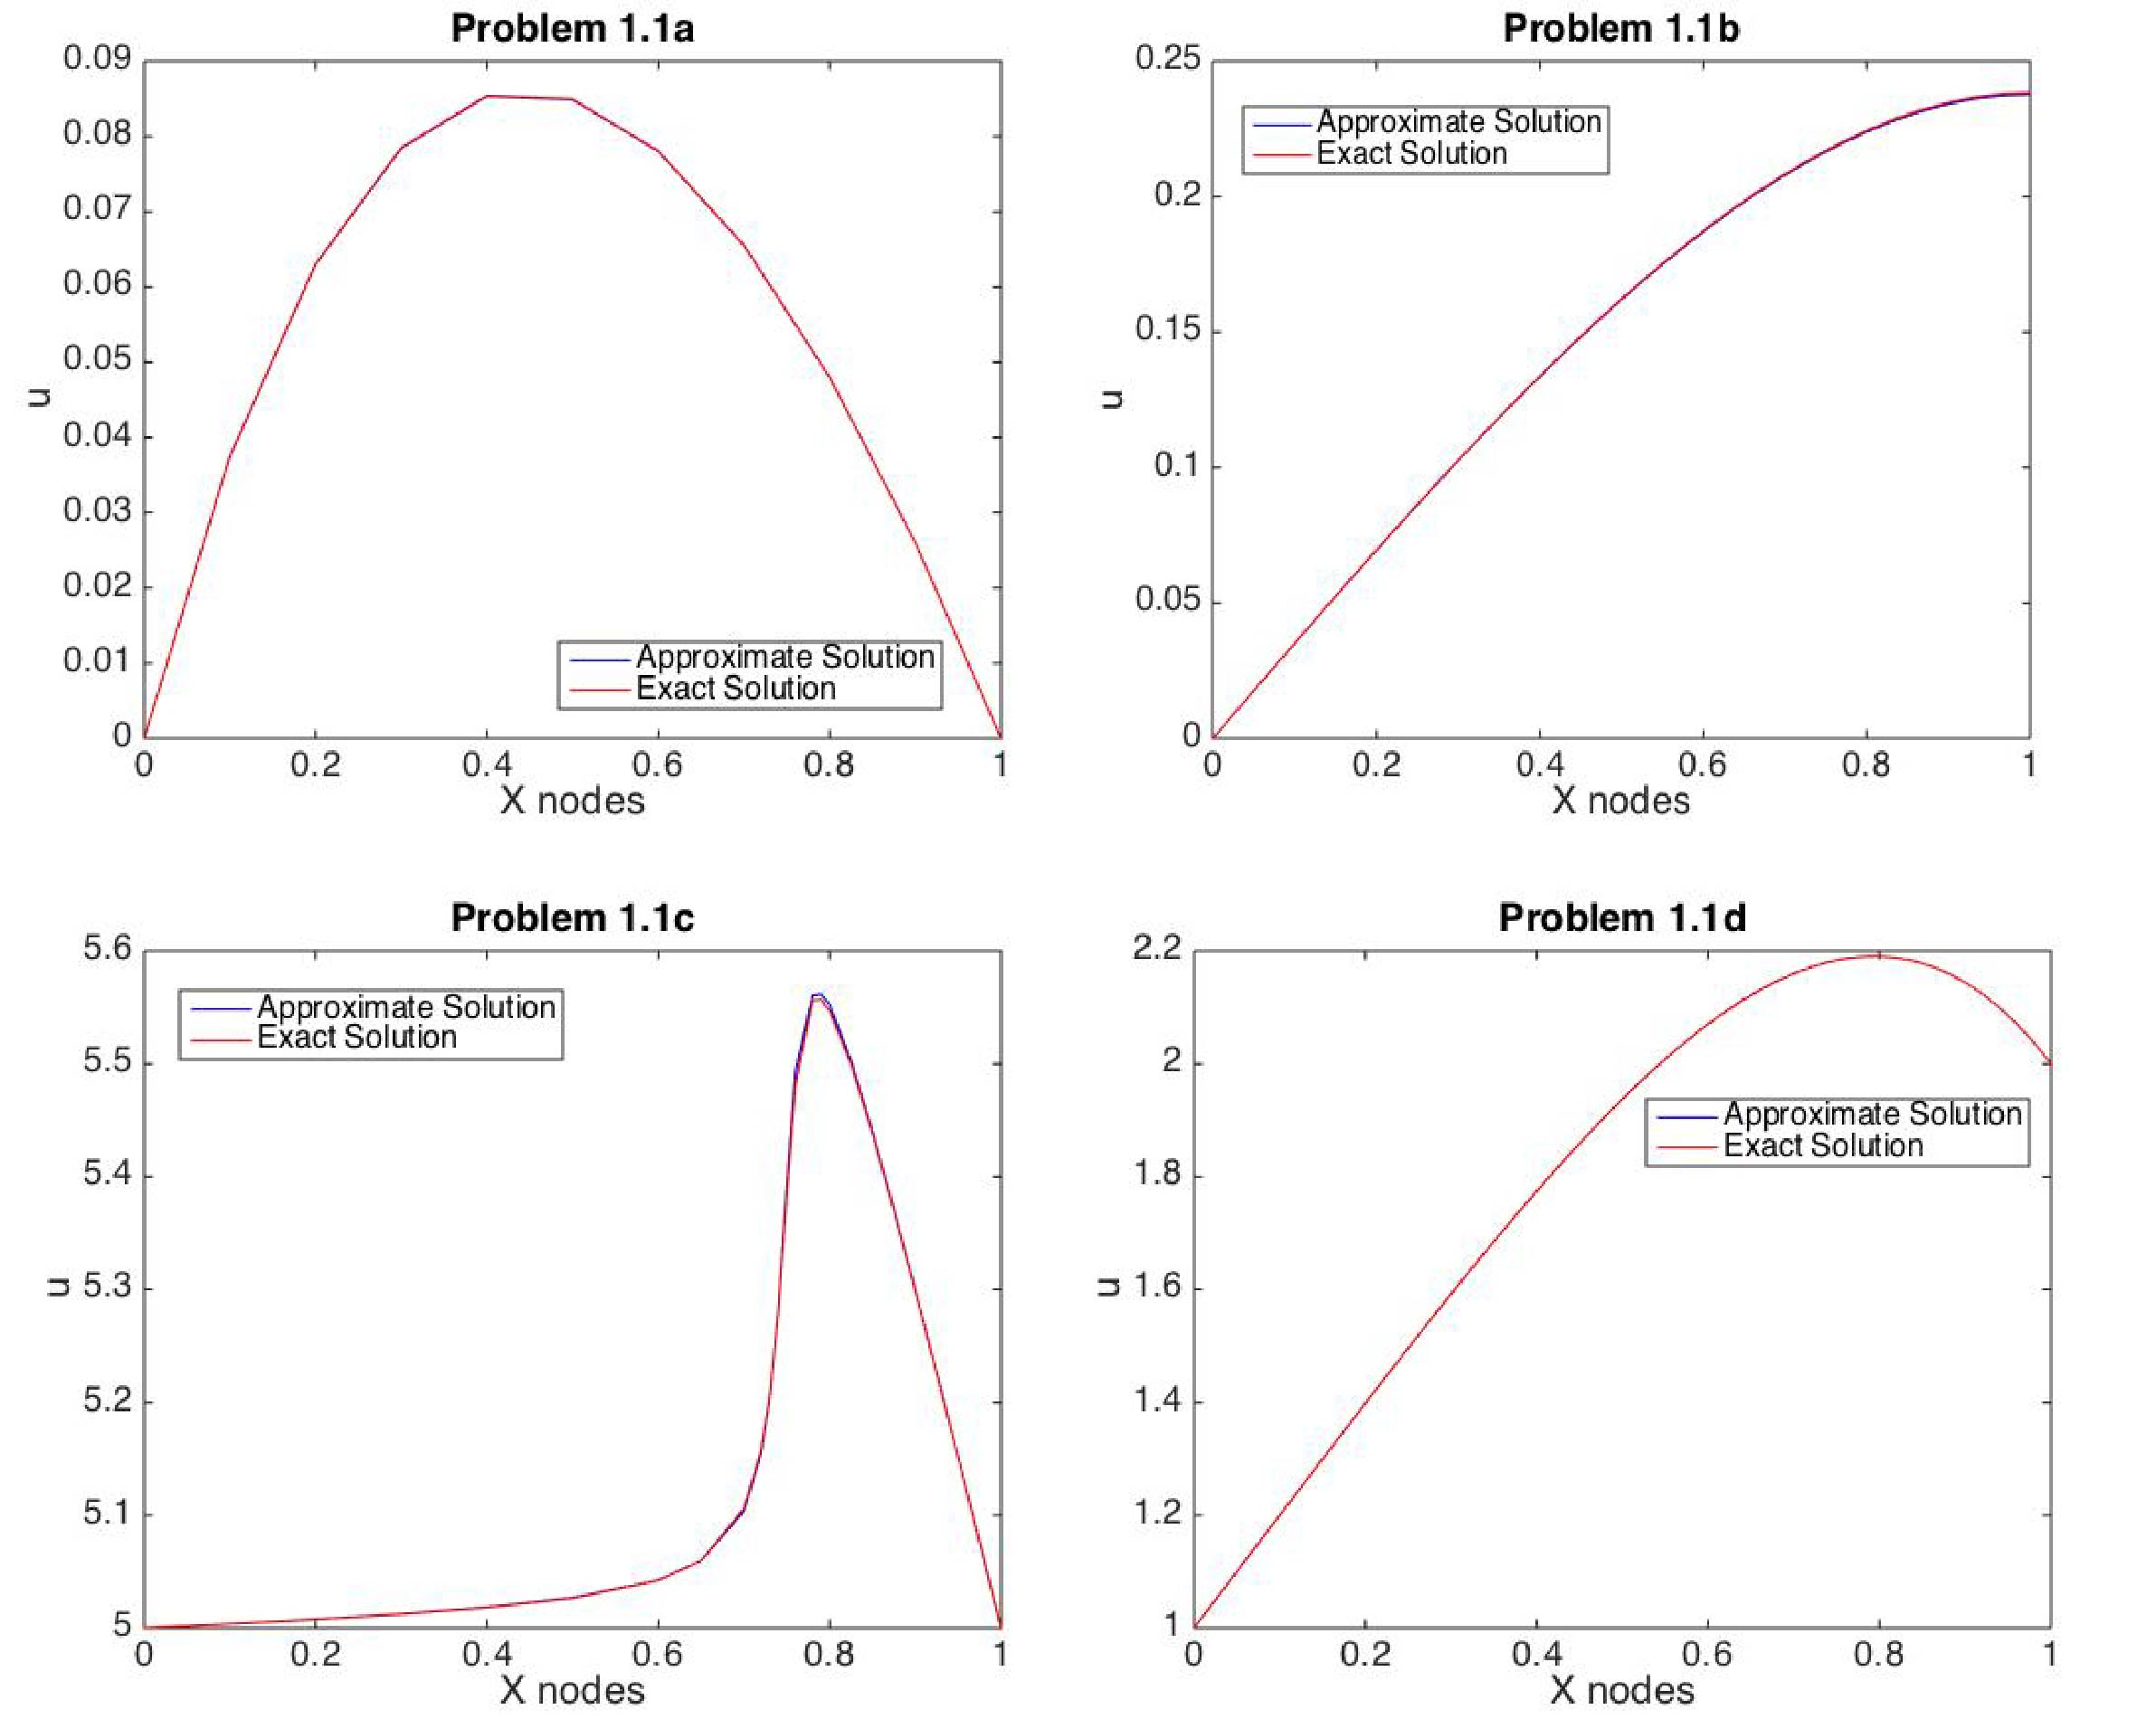
\includegraphics[width=\textwidth, keepaspectratio]{prob1.jpg}
\end{center}
% Problem 1.2 -------------------------------------------------------
\section*{Problem One Point Two}
\begin{enumerate}[(a)]
% 1.2a -------------------------------------------------------------
\item 
The strong form is given by:
\emph{Find $u\in C^2$ where}
\begin{gather*}
-\frac{d}{dr}(\kappa r\frac{du}{dr}) = rf\\
u(1) = 100,\;\;\; u(10) = 0
\end{gather*}

The weak form is derived at the end of the following steps:
\begin{gather*}
-\frac{d}{dr}(\kappa r\frac{du}{dr}) = rf\\
-\frac{d}{dr}(\kappa r\frac{du}{dr})\phi = rf\phi\\
-\rint{\frac{d}{dr}(\kappa r\frac{du}{dr})\phi} = \rint{rf\phi}\\
-\kappa\left(\phi r u_r\Big|_1^{10} - \rint{ru_r\phi_r}\right) = f\rint{r\phi}\\
\kappa\rint{ru_r\phi_r} = f\rint{r\phi}
\end{gather*}

% 1.2b --------------------------------------------------------------
\item If we are referring to \emph{relative error}, we get the desired accuracy with \texttt{Mesh 1}. The relative error at the indicated point is given by 
\begin{equation*}
\frac{|51.1219 - 48.8117|}{|51.1219|} = 0.0473 < \frac1{10}
\end{equation*}
There are 4 elements in this mesh. I'm quite sure that we are after the absolute error, however. we get the desired accuracy for \texttt{Mesh 4}.
\begin{equation*}
|(u - u_h)(3.25)| = |48.8679 - 48.8117| = 0.0562 < \frac1{10}
\end{equation*}
There are 32 elements in this mesh.
% 1.2c --------------------------------------------------------------
\item Here is the plot:
\begin{center}
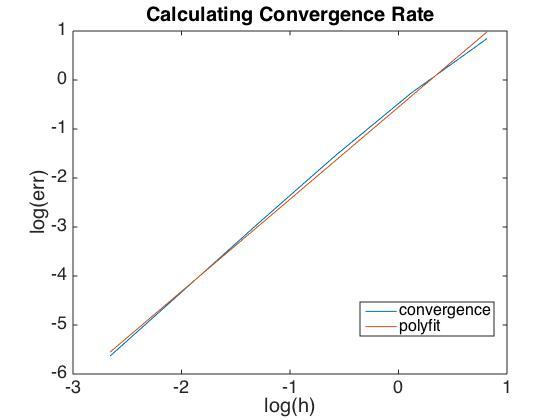
\includegraphics[width=0.5\textwidth]{prob12b.jpg}
\end{center}
Here is the code for plotting:
\begin{lstlisting}
err = fliplr(log([2.3102 0.7667 0.2162 0.0562 0.0142 0.0036]));
h = fliplr(log([2.25 1.125 0.5625 0.281250 0.140625 0.070312]));
p = polyfit(h, err, 1); % Fit to a line
disp(p(1));
P = polyval(p, h);
set(gcf, 'color', 'w')
plot(h, err, h, P)
title('Calculating Convergence Rate')
xlabel('log(h)')
ylabel('log(err)')
legend('convergence', 'polyfit')
\end{lstlisting}

The slope of the line given by \texttt{polyfit()} is $1.8811 \approx 2$.	

% 1.2d --------------------------------------------------------------
\item The absolute error in this example is $0.0459 < \frac1{10}$ at the indicated point. There are, however, only 10 elements, which is fewer than the 32 used in the structured mesh in part (b). The nodes are spaced more closely around $r = 3.25$ in the unstructured mesh than in some of the structured meshes with more elements, and therefore gives a better approximation in this neighborhood. 

Also, the solution is nearly linear in the right half of the domain, and so the solutions rapidly converge  point-wise for all meshes in this subdomain.  The unstructured mesh has nodes at only $x = 5.5$ and $x = 7.375$ and one of the structured meshes has nodes at $x = 6.625$, $x = 7.1875$, $x =7.75$, and $x =8.31$, yet both have similar accuracies in this neighborhood.
% 1.2e --------------------------------------------------------------
\item For this problem, I will use a finite difference to approximate $u_h'$ at the end points. That is, the derivative is approximated as
\begin{equation*}
u_h' = \frac{u^{(e)}_l- u^{(e)}_r}{h^{(e)}}
\end{equation*}
where $e$ denotes `element', $l$ denotes `left' and $r$ denotes `right' for the left and right endpoints of the element. Since we are looking for $10\%$ error, I assume that in this case we are referring to relative error and not absolute error. At the left endpoint I get the desired accuracy with \texttt{Mesh 5}. At the right endpoint I get the desired accuracy with \texttt{Mesh 2}.
% 1.2f --------------------------------------------------------------
\item The convergence of the flux is slower than the convergence for the solution. The rates of convergence are about $0.7847$ and $1.1516$ at the left and right endpoints, respectively. 
\begin{center}
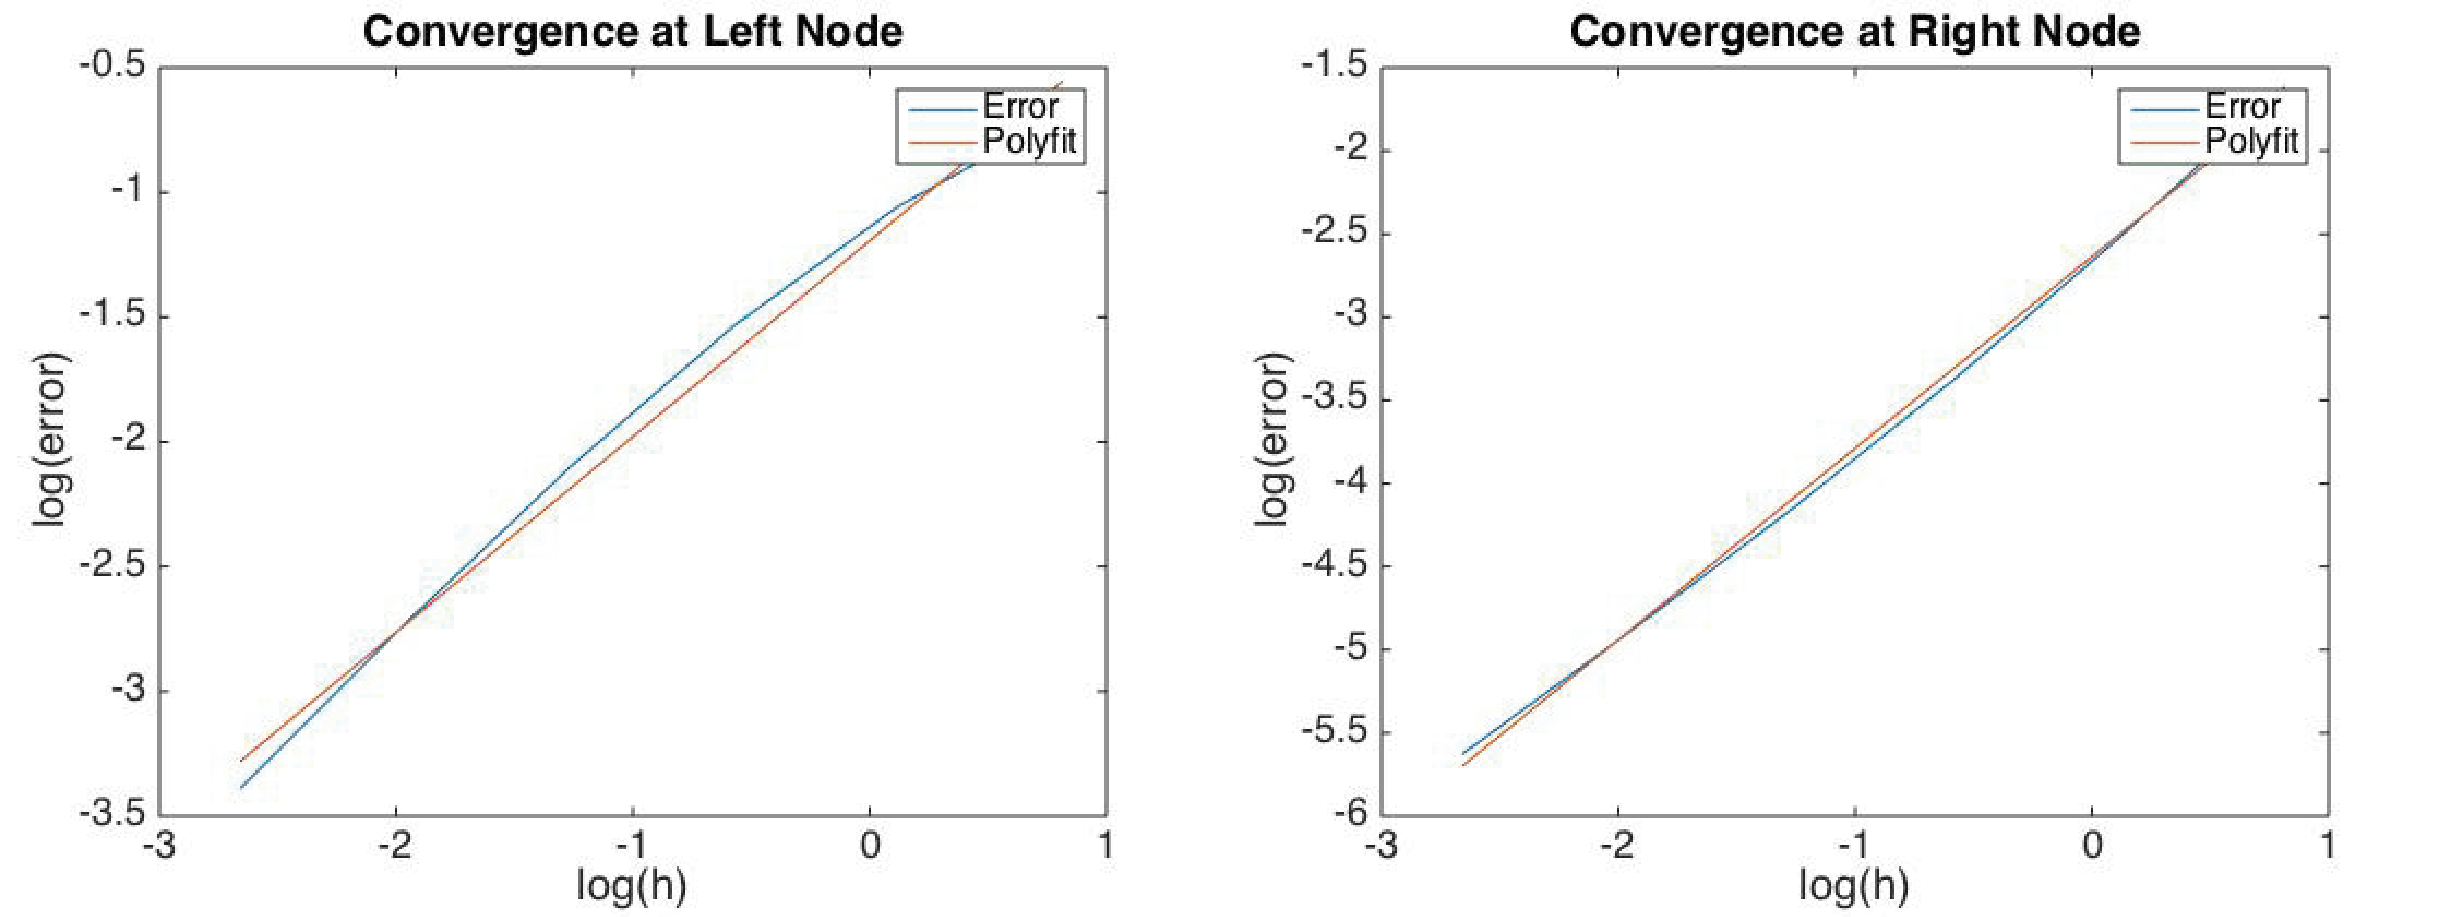
\includegraphics[width=\textwidth]{convergence.png}
\end{center}
\end{enumerate}
% Problem 2.1 -------------------------------------------------------
\section*{Problem Two Point One}
\begin{enumerate}[(a)]
\item

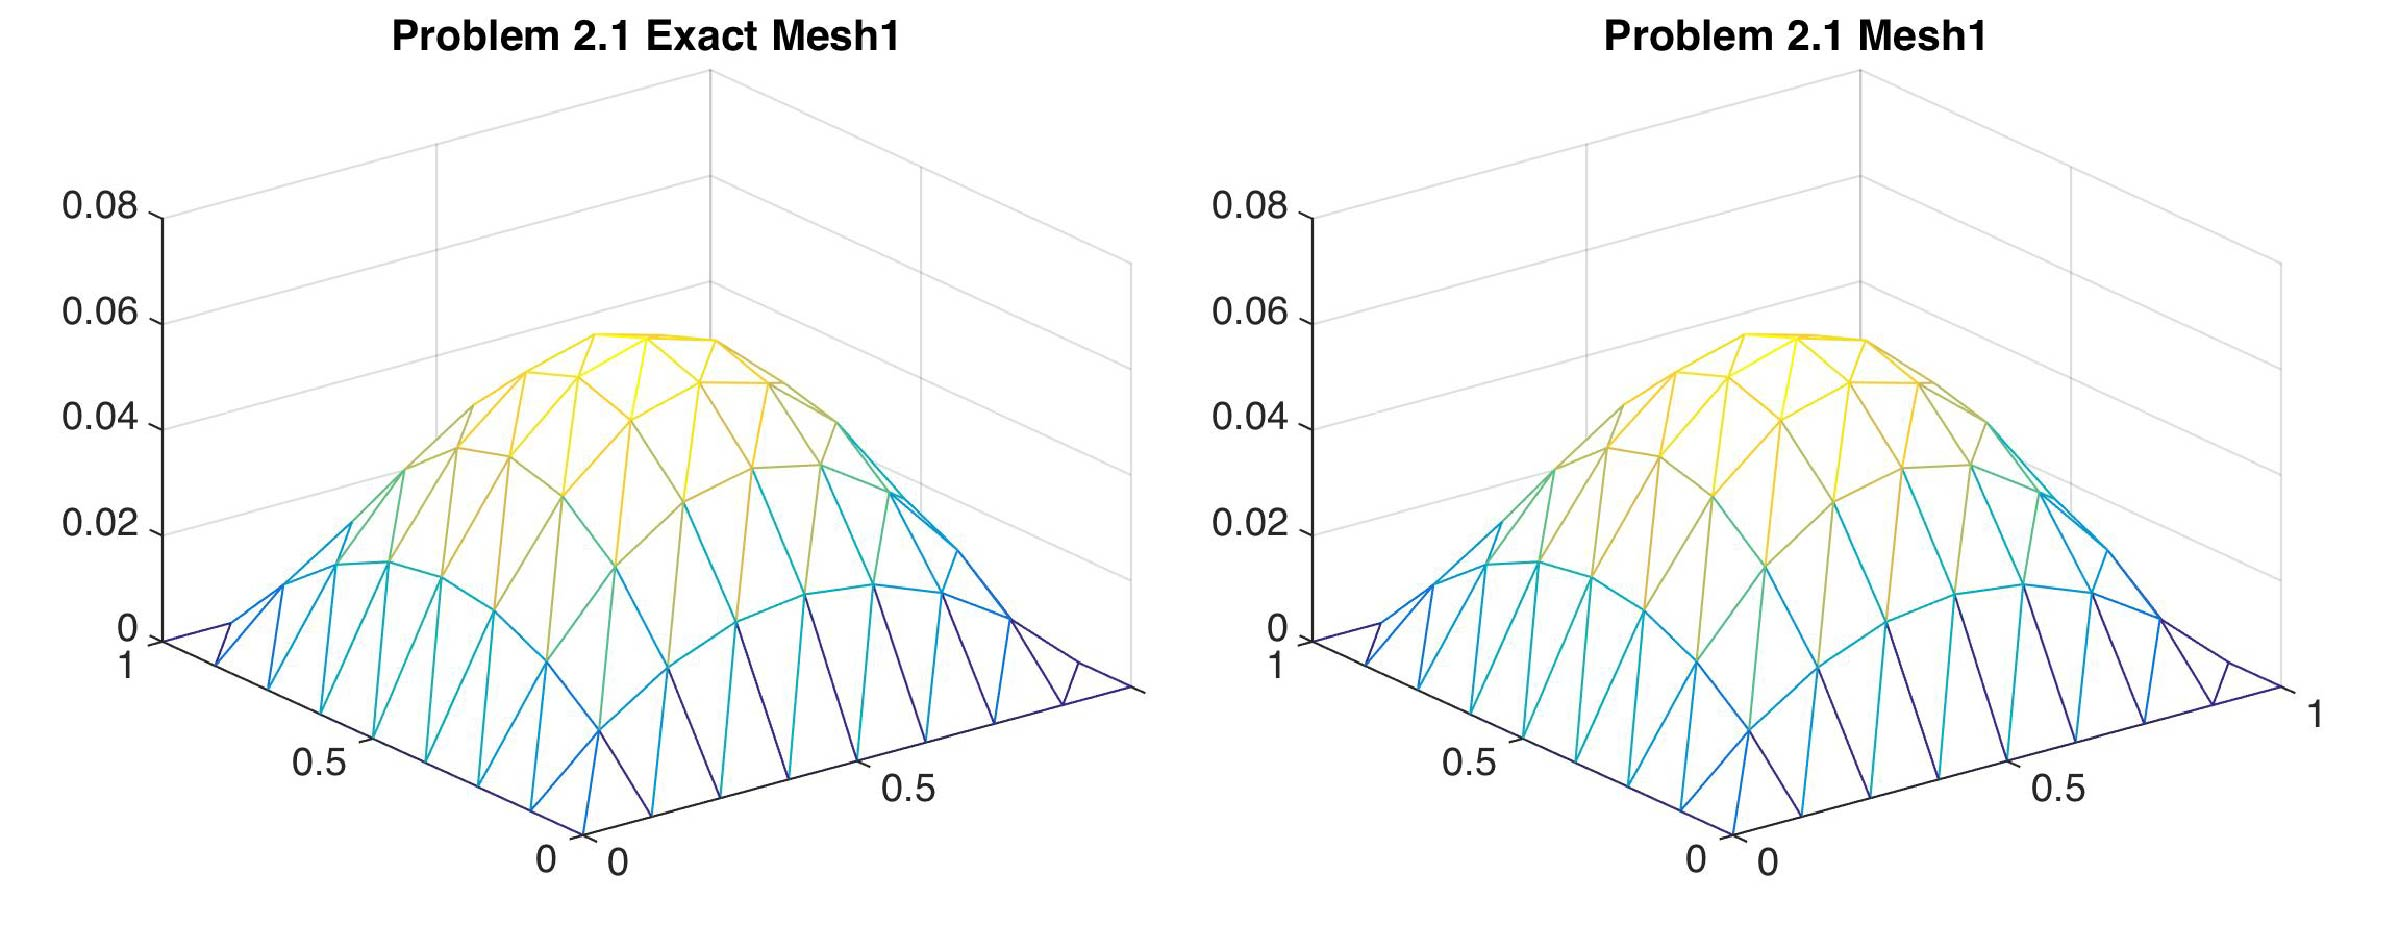
\includegraphics[width=\textwidth]{211.jpg}
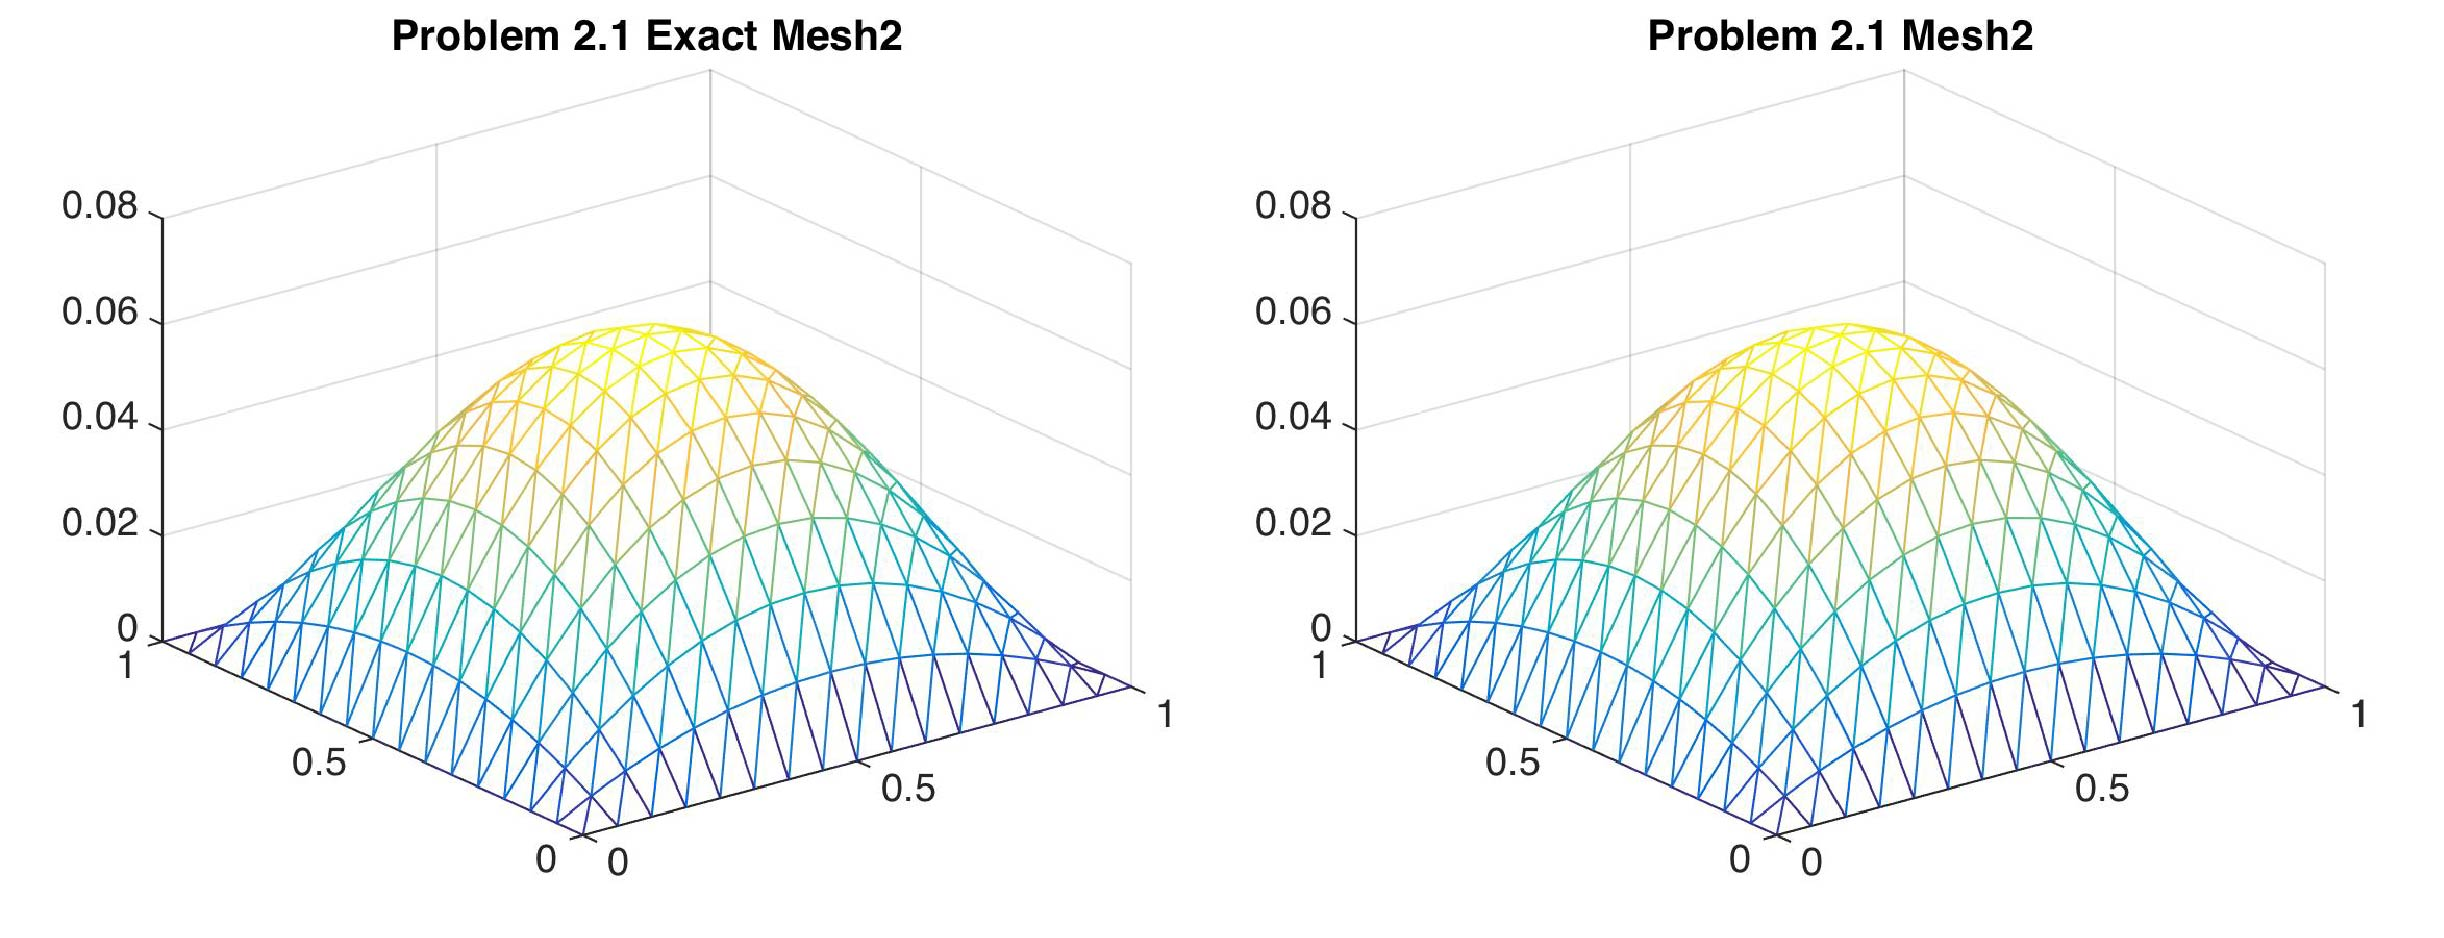
\includegraphics[width=\textwidth]{212.jpg}
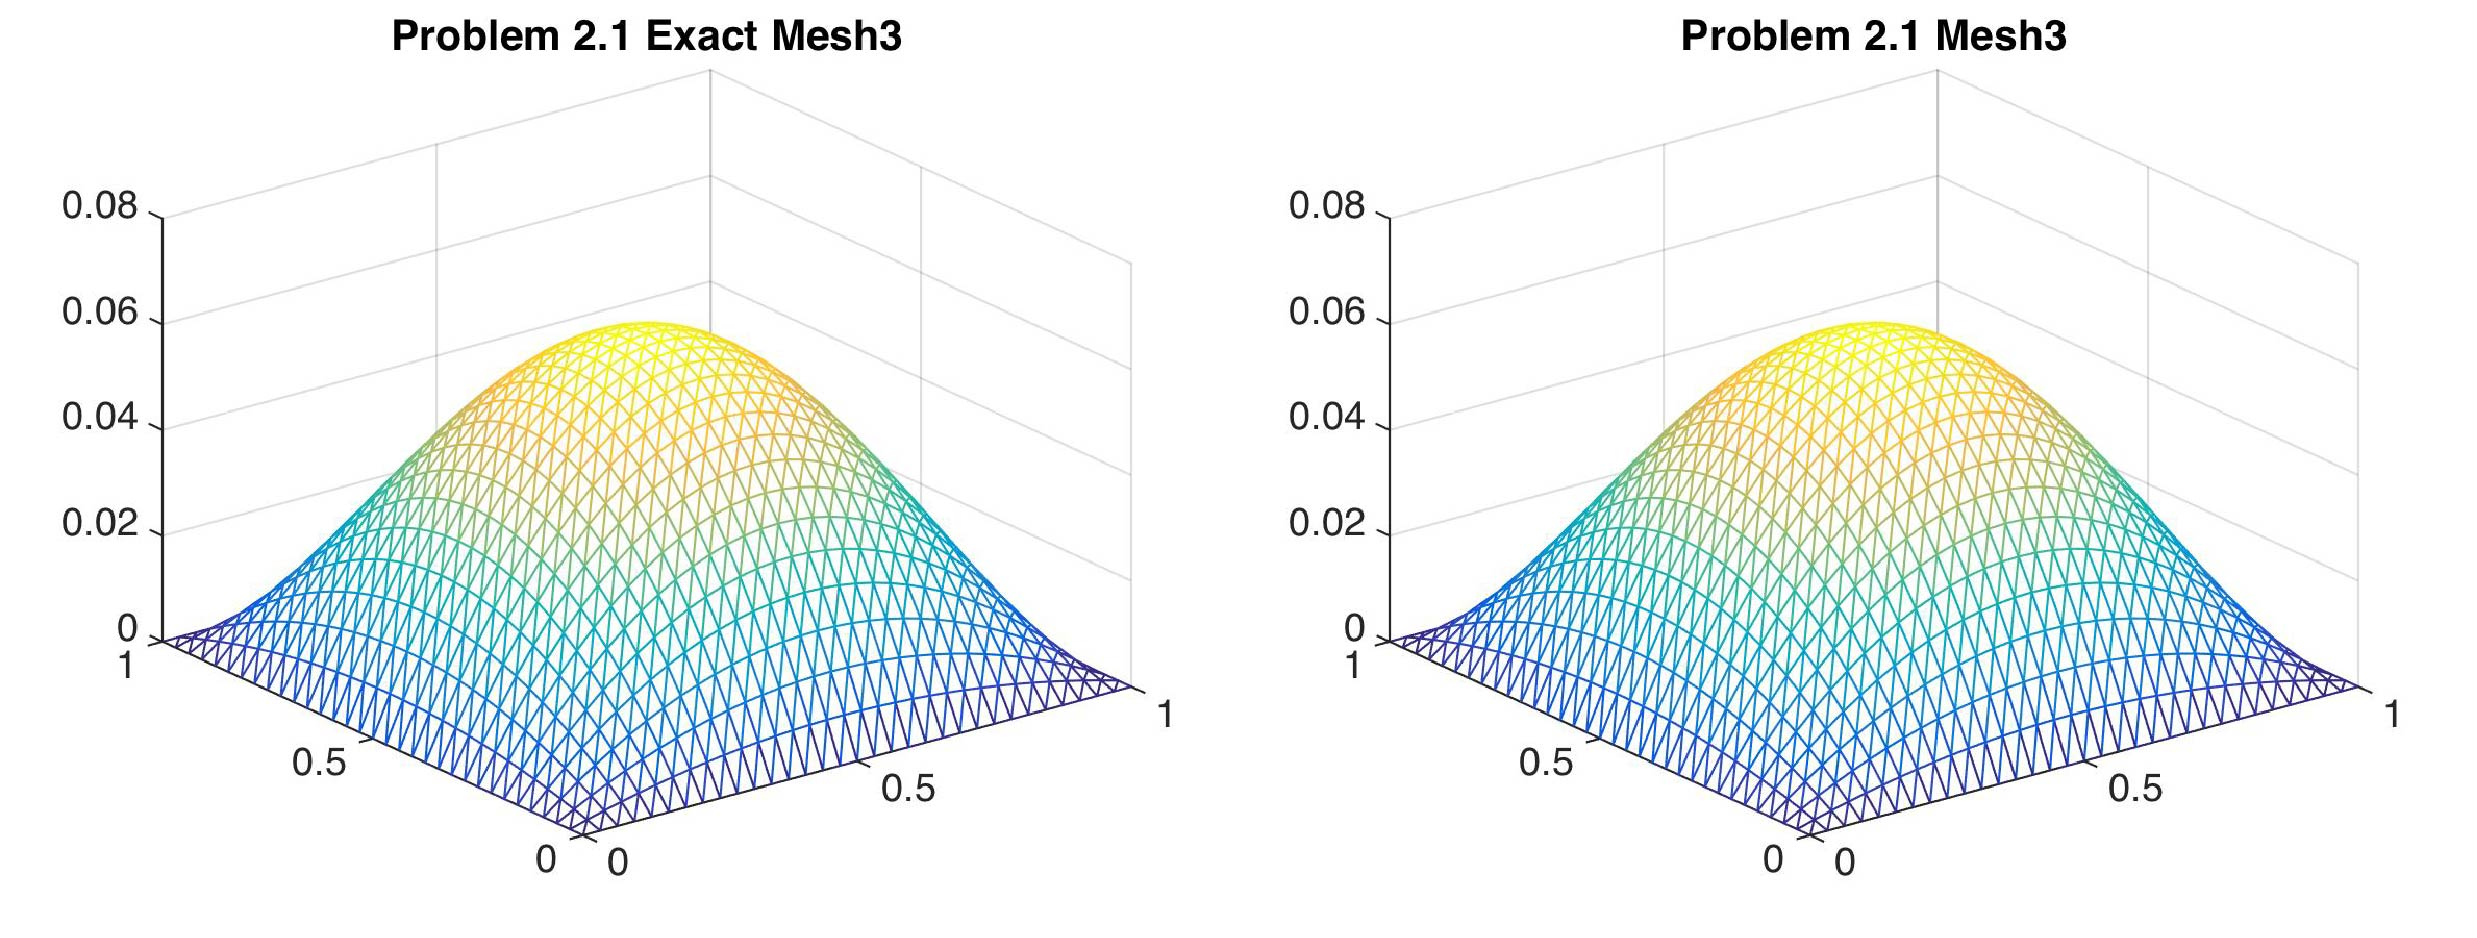
\includegraphics[width=\textwidth]{213.jpg}
\item
Mesh 1: L2 = 1.593564e-03; Linf = 3.433228e-03;
Mesh 2: L2 = 4.044021e-04; Linf = 9.164810e-04;
Mesh 3: L2 = 1.014799e-04; Linf = 2.365708e-04;

\item 
For this step and for the next step our $h$ is the length of the longest edge in the triangular  element. We get the proper second order convergence as the $h$ shrinks, as demonstrated in the following table:

\begin{center}
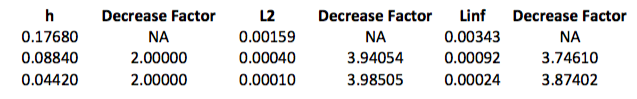
\includegraphics[width=0.9\textwidth]{21b.png}
\end{center}

\item

\begin{center}
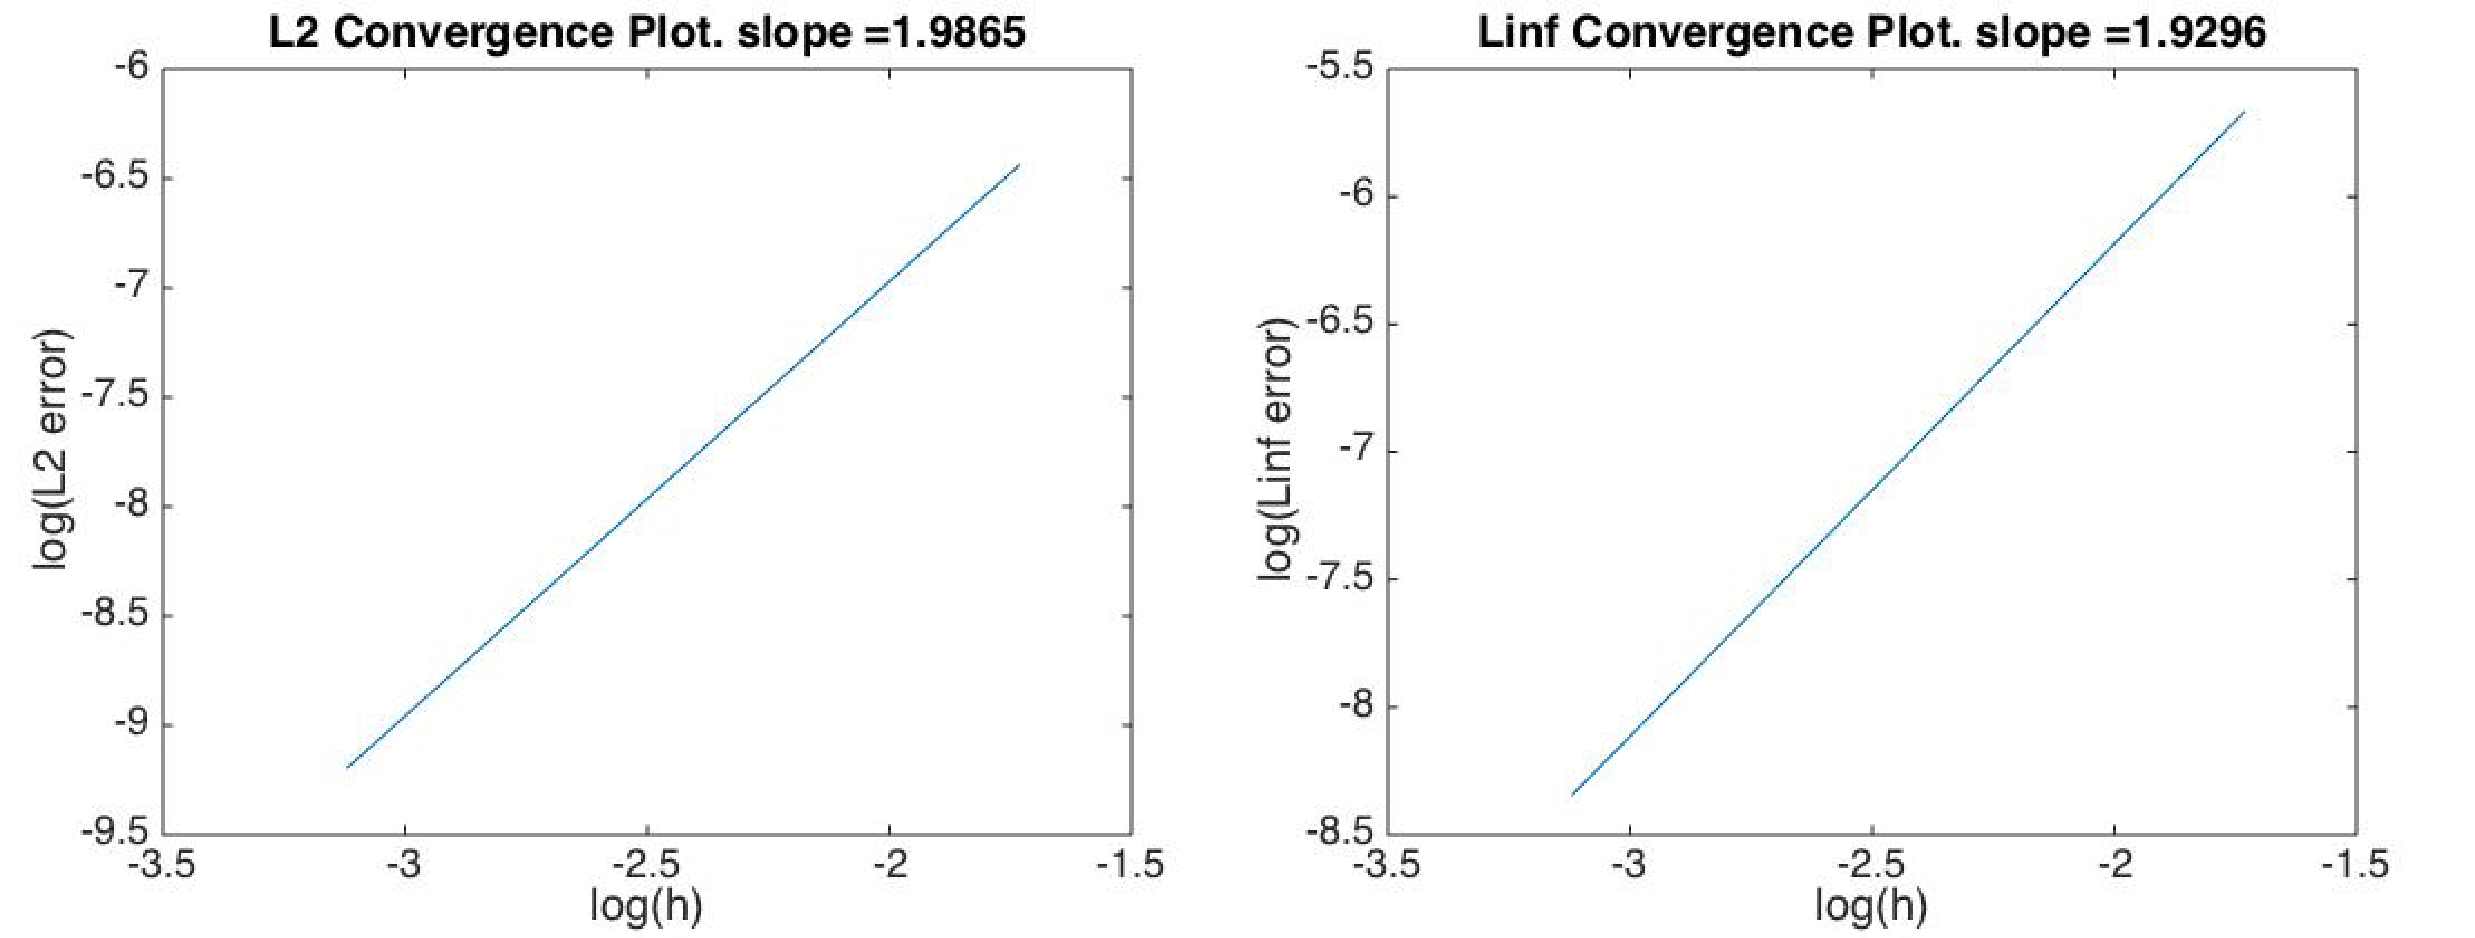
\includegraphics[width=0.9\textwidth]{err.png}
\end{center}

\item

\begin{center}
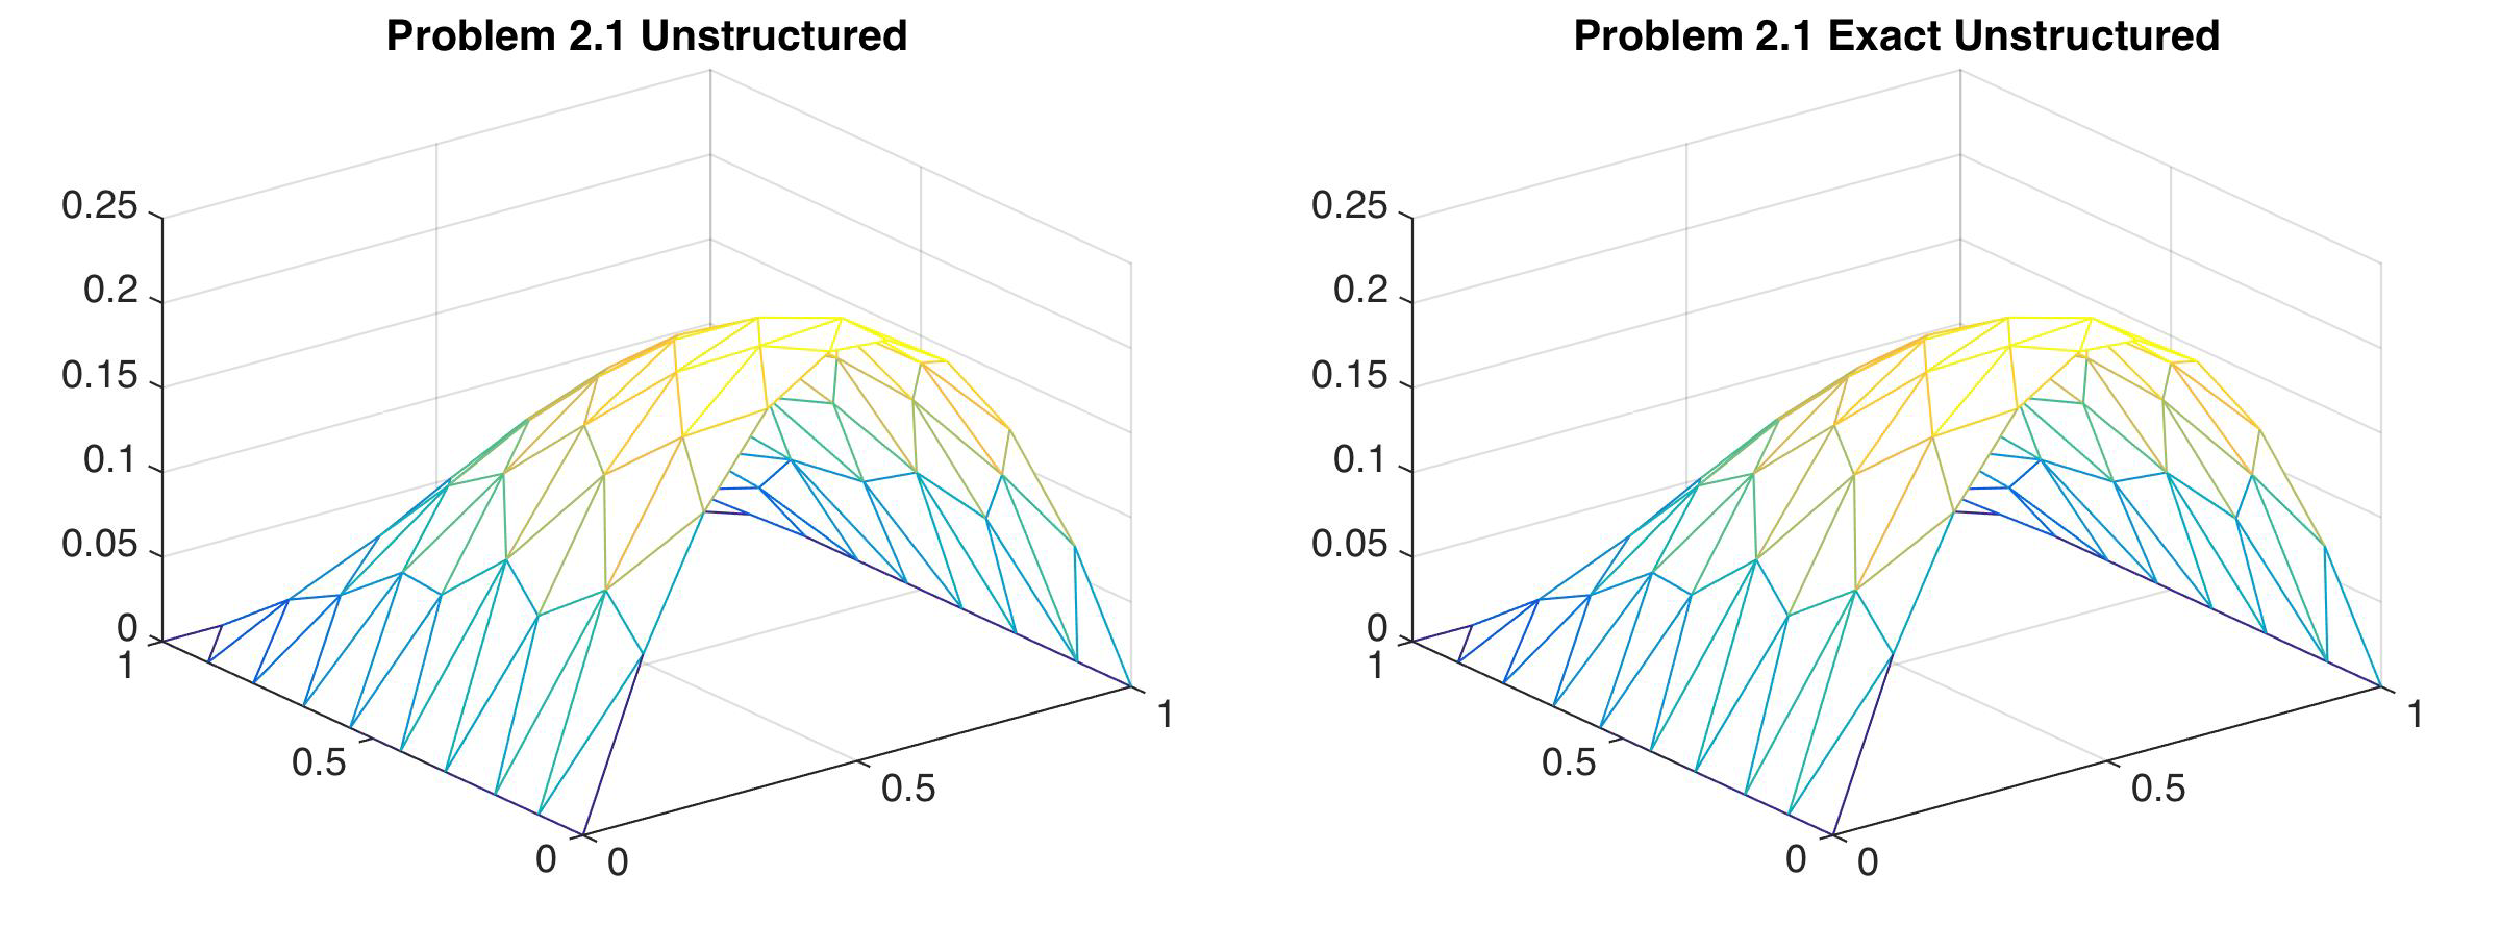
\includegraphics[width=0.9\textwidth]{21du.png}
\end{center}

\begin{center}
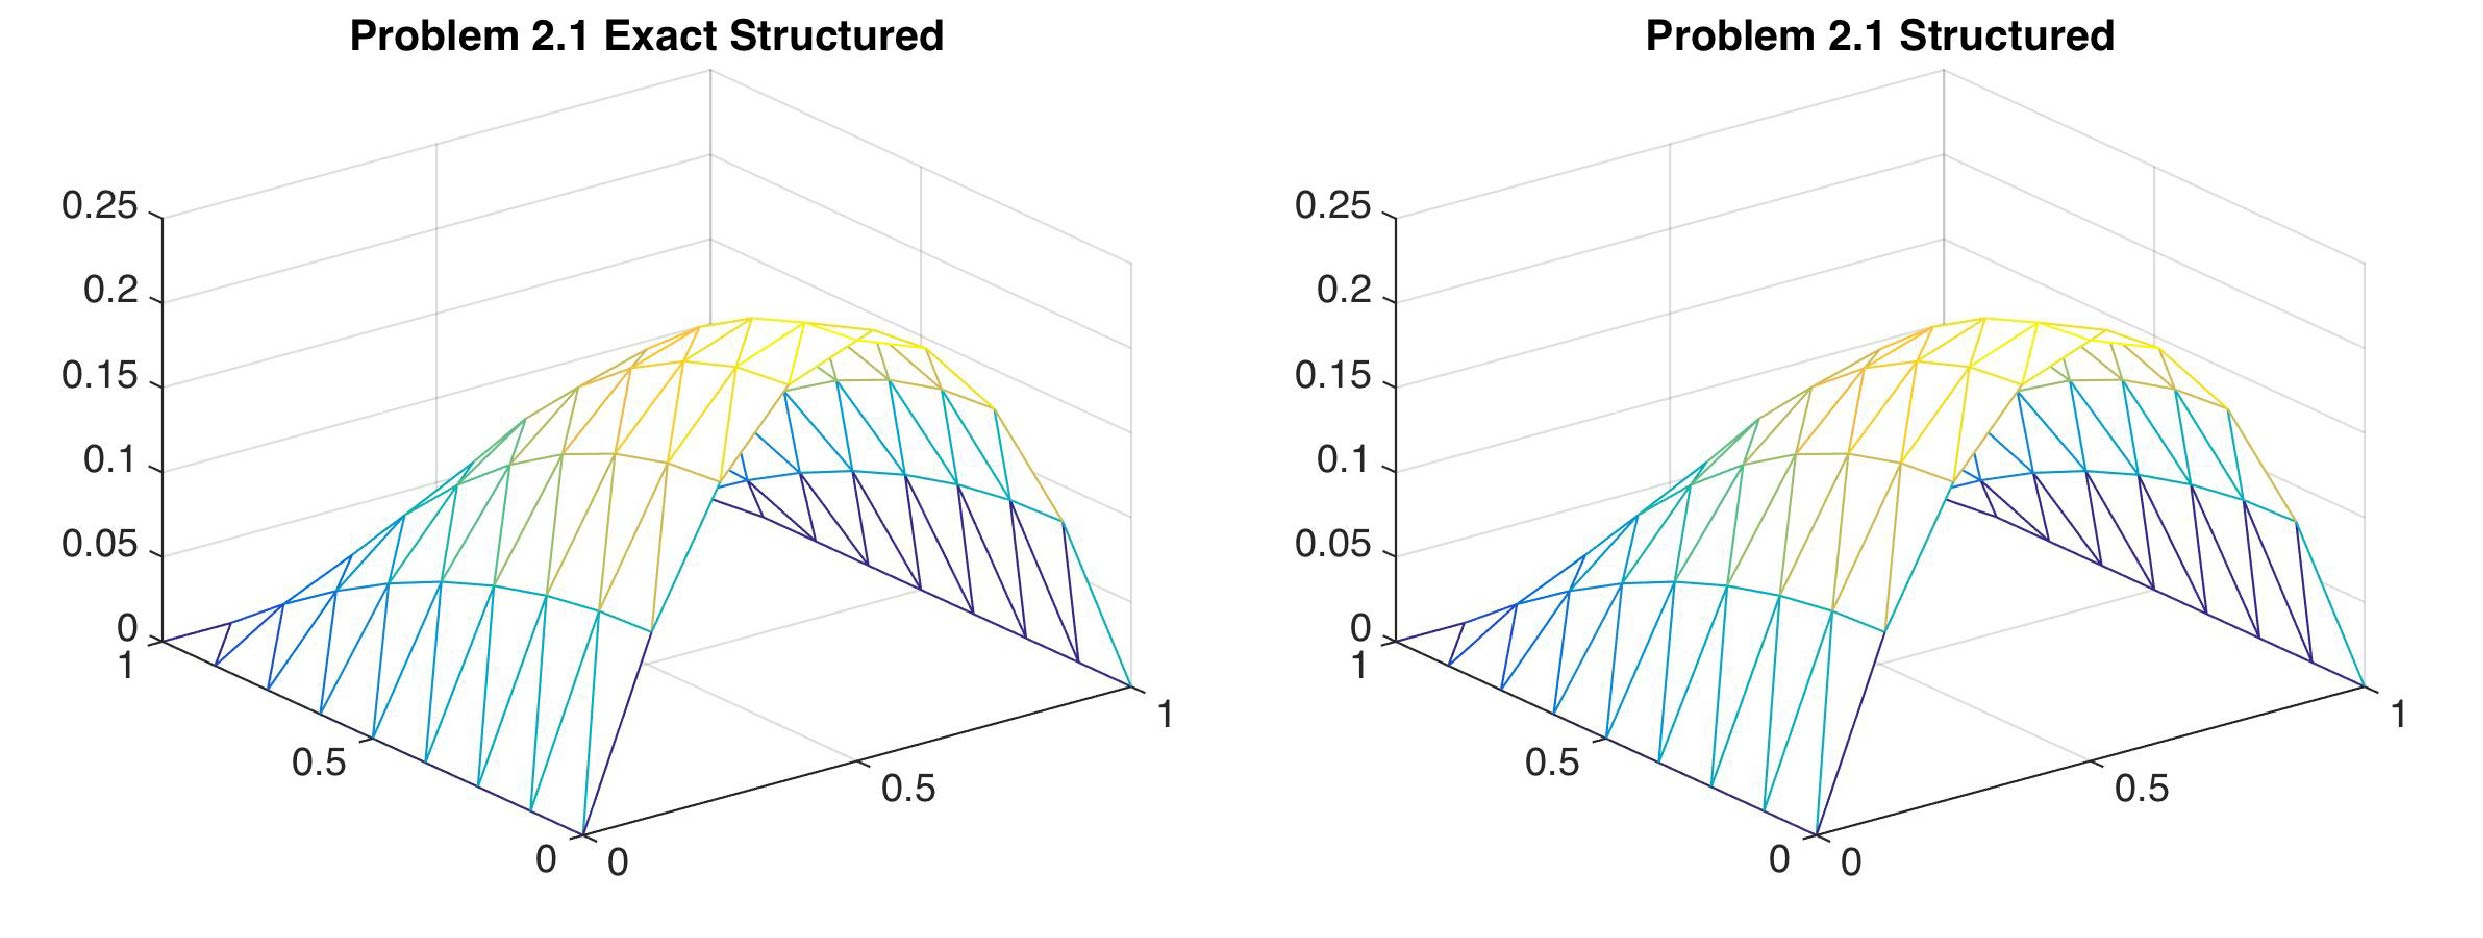
\includegraphics[width=0.9\textwidth]{21ds.jpg}
\end{center}

\item
The unstructured mesh gives the following error norms: L2 = 8.916471e-06, Linf = 6.581145e-03;

And the structured mesh gives the following: 	L2 = 1.340423e-05, Linf = 7.186729e-03;

The structured mesh gives an error marginally higher than the error of the unstructured mesh. The structured mesh has 128 elements, and the unstructured mesh has 131 elements, so the marginal improvement in error might come from this fact. The error analysis we conducted in class was independent of the connectivity of the mesh we used, so initially I did not expect to see any difference. However, since the mesh we use is made up of mostly equilateral triangles, and since there are slightly more triangles, we should expect the maximal edge length of an element, $h$ to be smaller in the unstructured mesh than in the structured mesh. 

Another thought that occurred to me was that the unstructured mesh could have terrible accuracy if some elements were made too big, but we don't have to worry about that in this case. We should expect most of the elements in the unstructured mesh to have relatively the same size, since the length of an edge shared by two elements has the same length in both elements, and then this approximate  edge length extends to all of the edges in the mesh by the transitive property of equality, coupled with the fact that all triangles are nearly equilateral.
 
\end{enumerate}
% Problem 2.2 -------------------------------------------------------
\section*{Problem Two Point Two}
\begin{enumerate}[(a)]

\item
\begin{center}
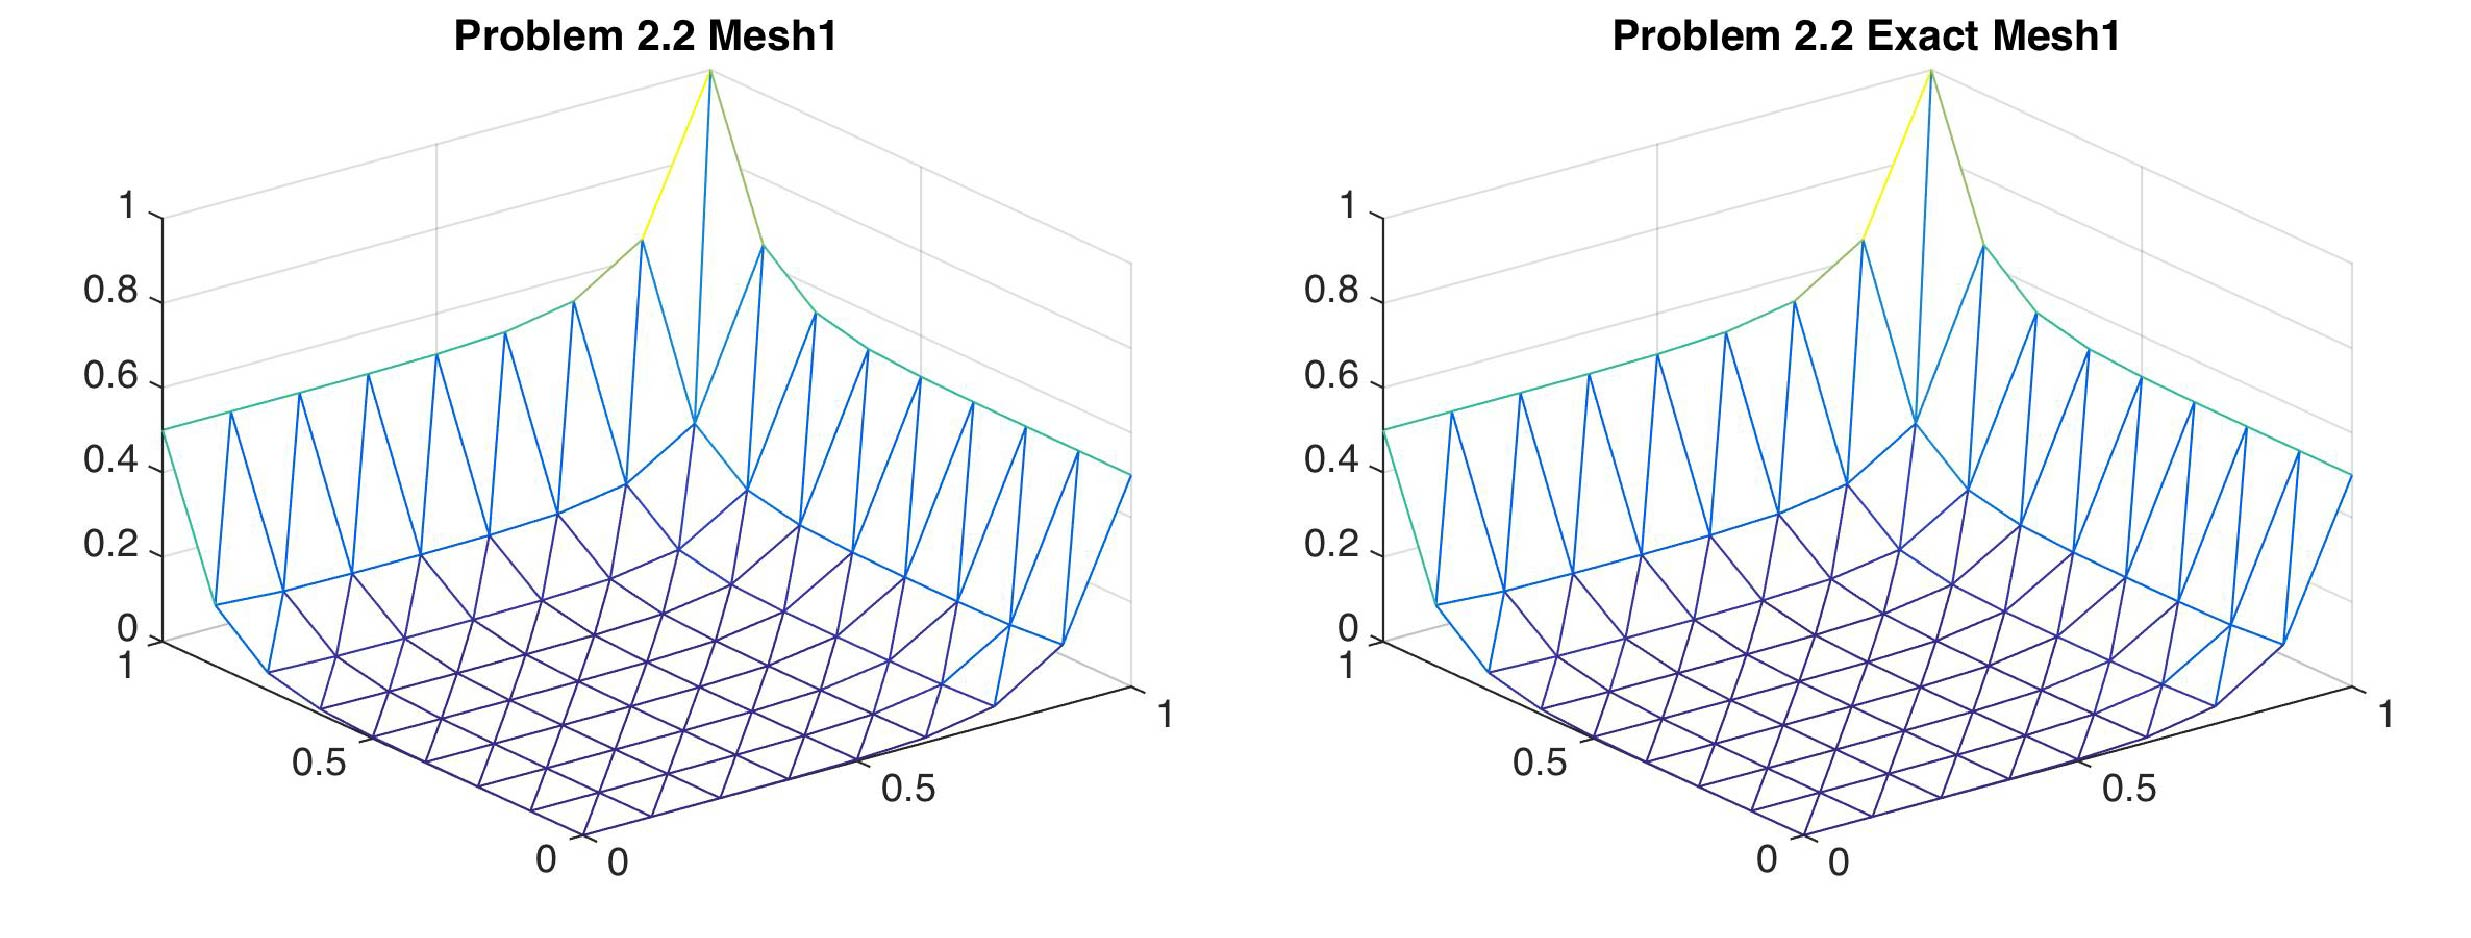
\includegraphics[width=0.9\textwidth]{P221.jpg}
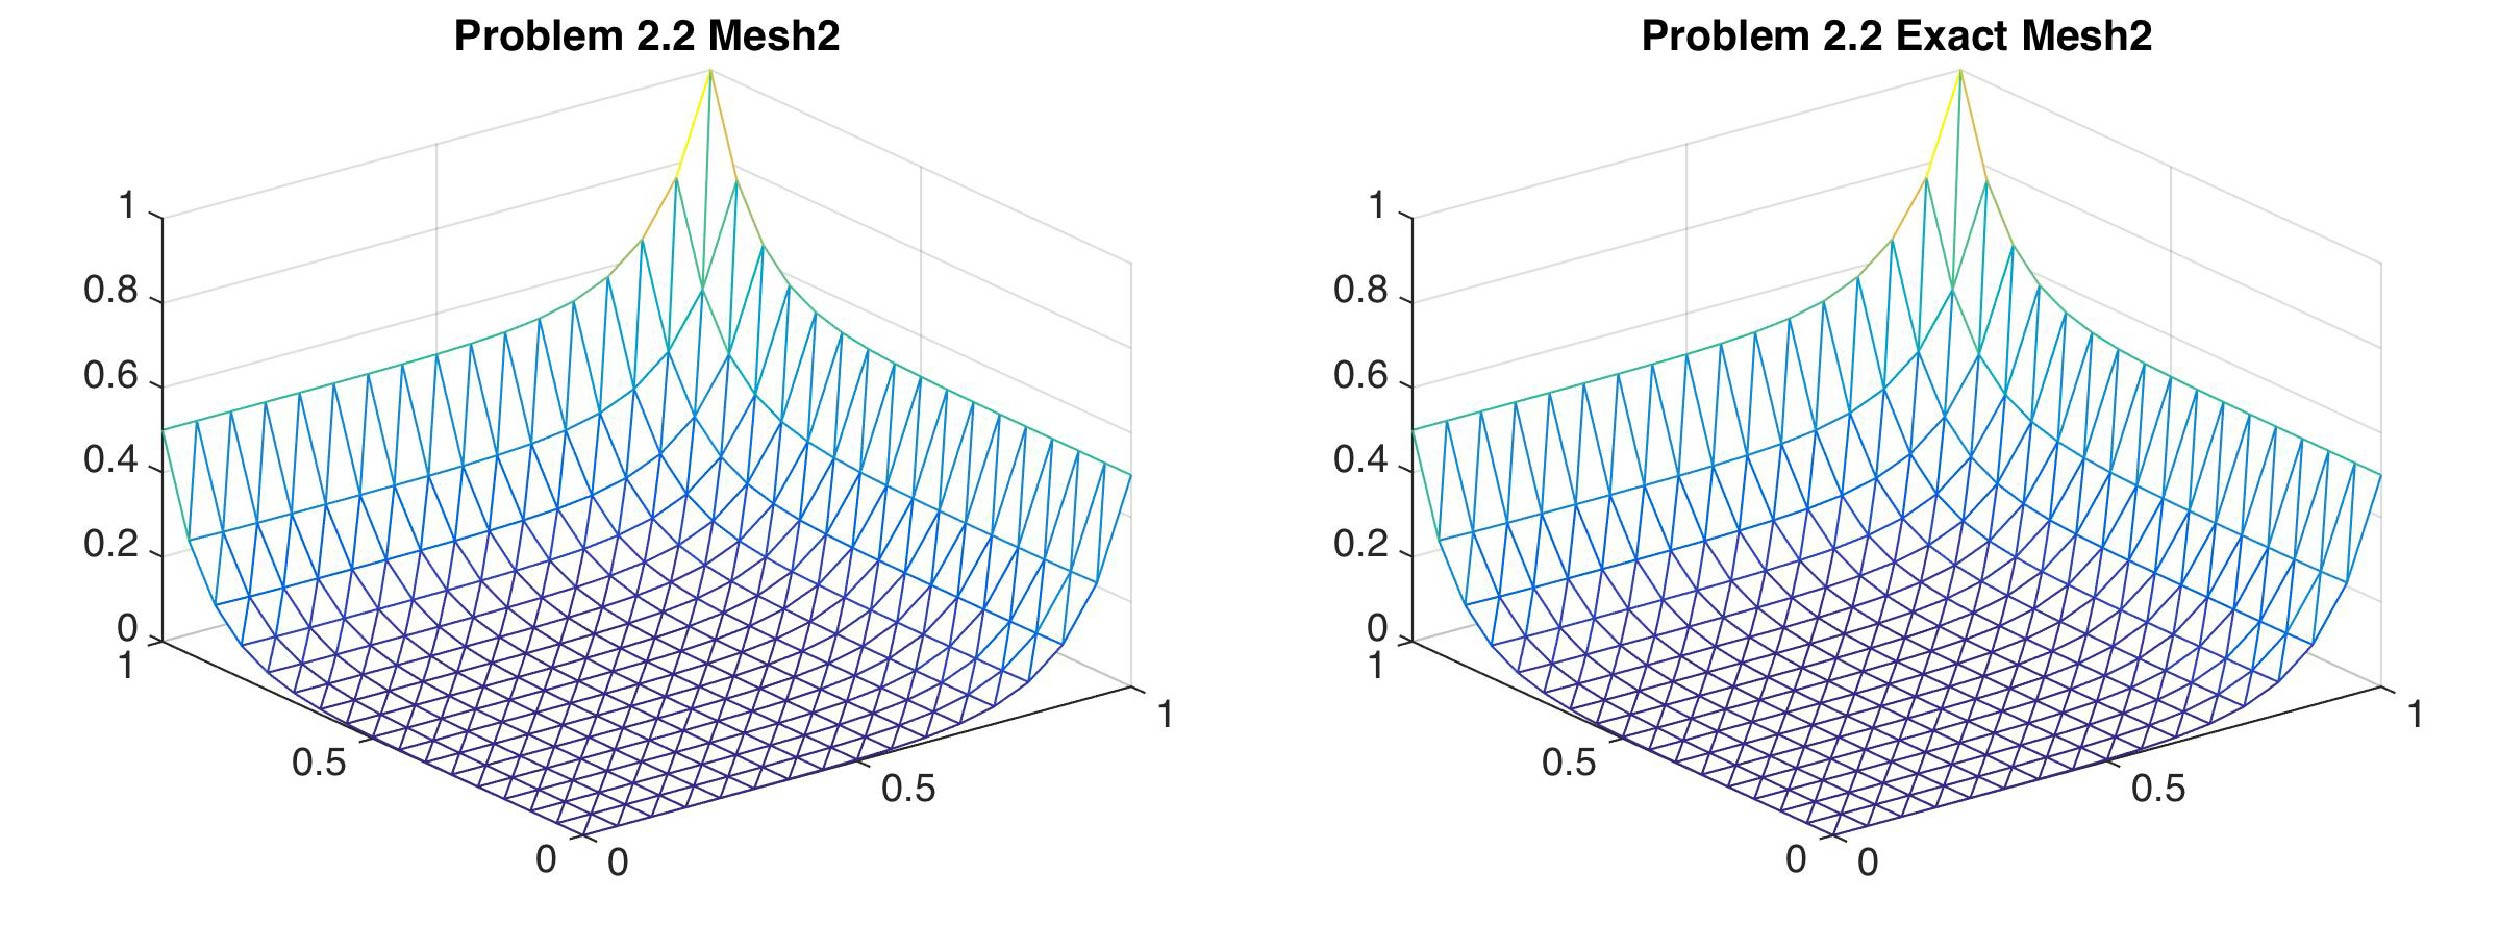
\includegraphics[width=0.9\textwidth]{p222.jpg}
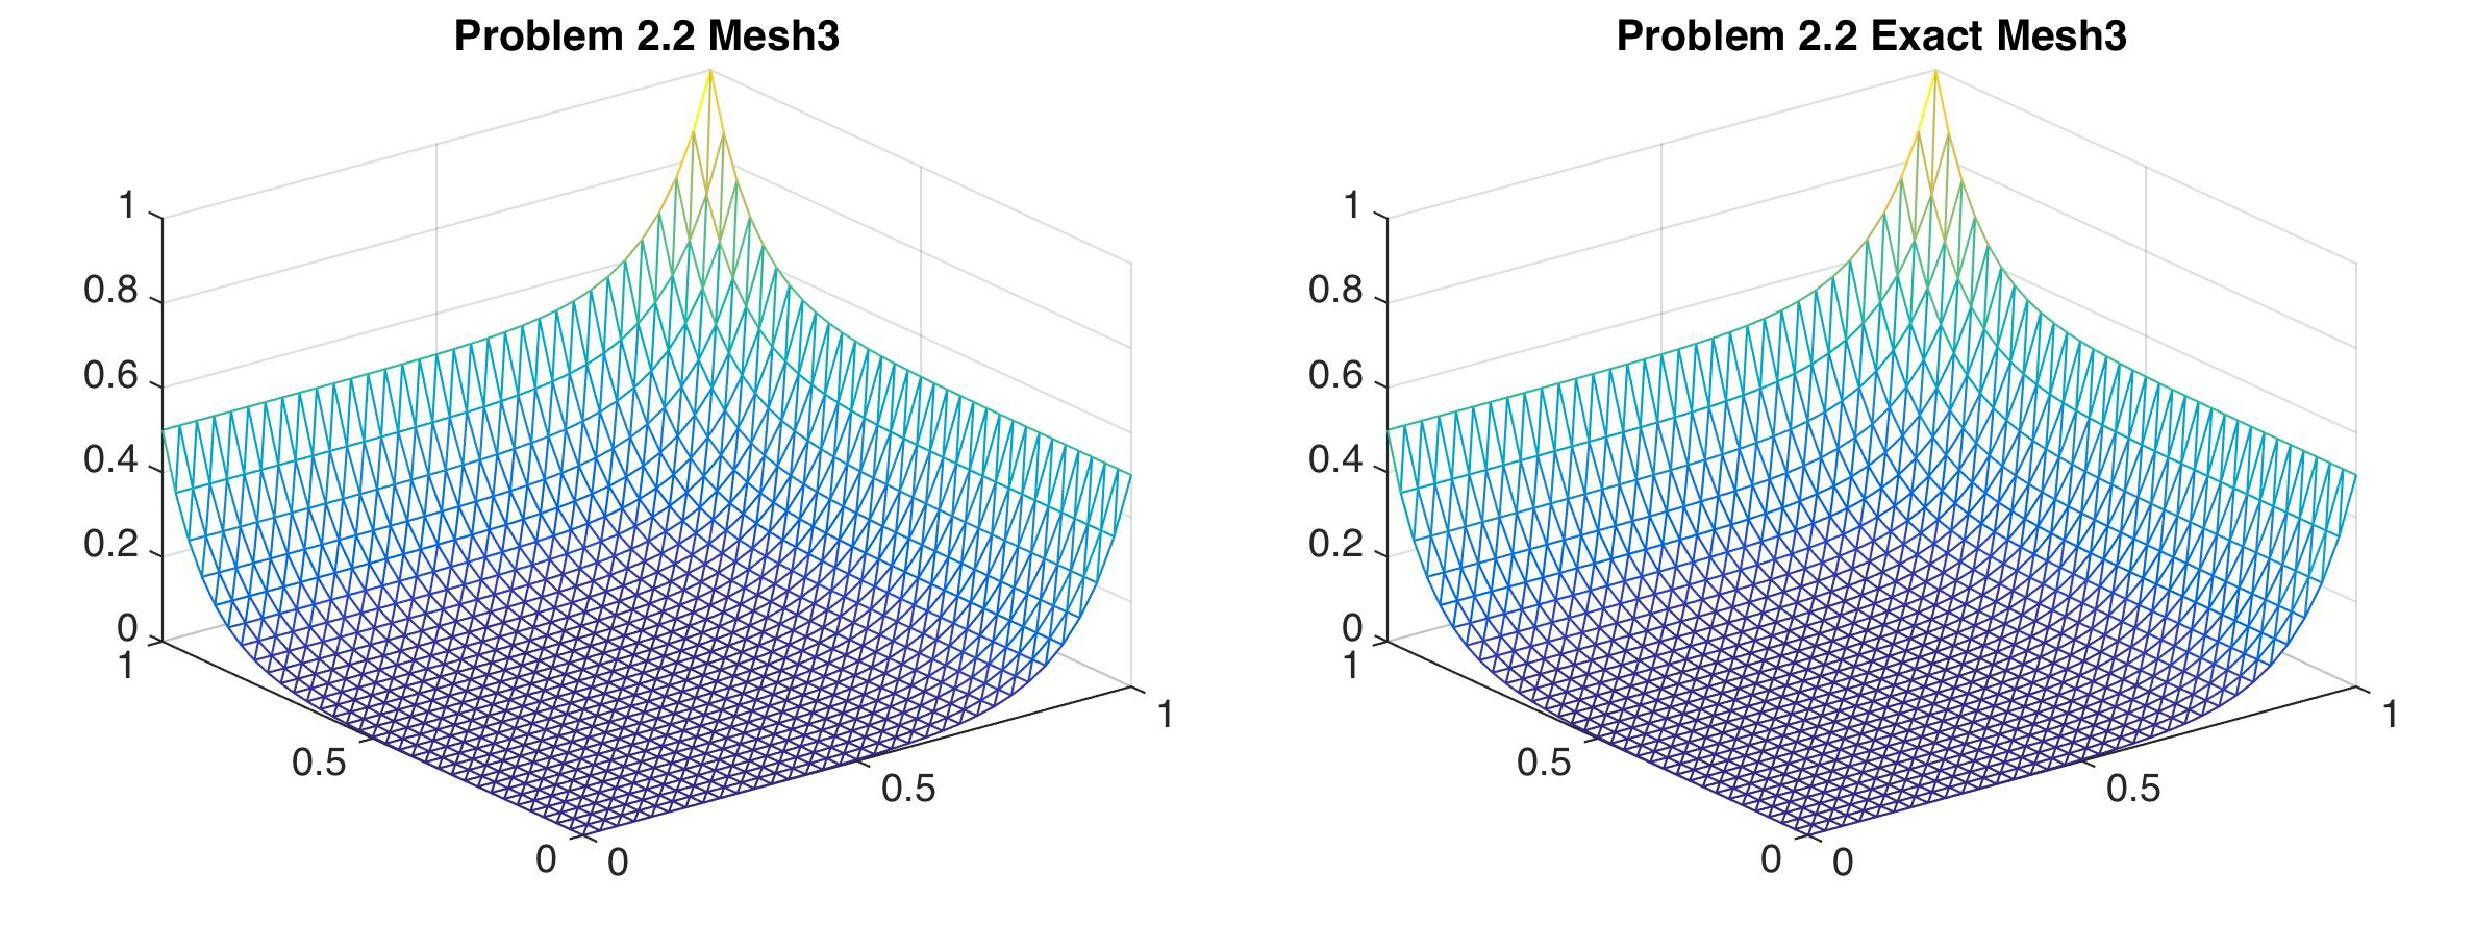
\includegraphics[width=0.9\textwidth]{p223.jpg}
\end{center}

\texttt{tic} and \texttt{to} were used to time the part of the code which calculates the approximate $u$. \texttt{Mesh 1} ran in 0.1292 seconds, \texttt{Mesh 2} ran in 0.306532 seconds, and \texttt{Mesh 3} ran in 8.369406 seconds.

\item There are no oscillations and this is not surprising. There is no advection term in the problem.

\item
The error norms for the different meshes  are:\\
Mesh 1: L2 = 2.116320e-02; Linf = 9.736566e-02;\\
Mesh 2: L2 = 5.608765e-03; Linf = 3.422807e-02;\\
Mesh 3: L2 = 1.422964e-03; Linf = 1.023980e-02;

\item The solution shows the proper convergence in the $L^2$ norm, but the rate is not as high as we want in the infinity norm. This could be due to the way we define $h$. The convergence rate rounds up to 2, so it is nothing to worry too much about.


\begin{center}
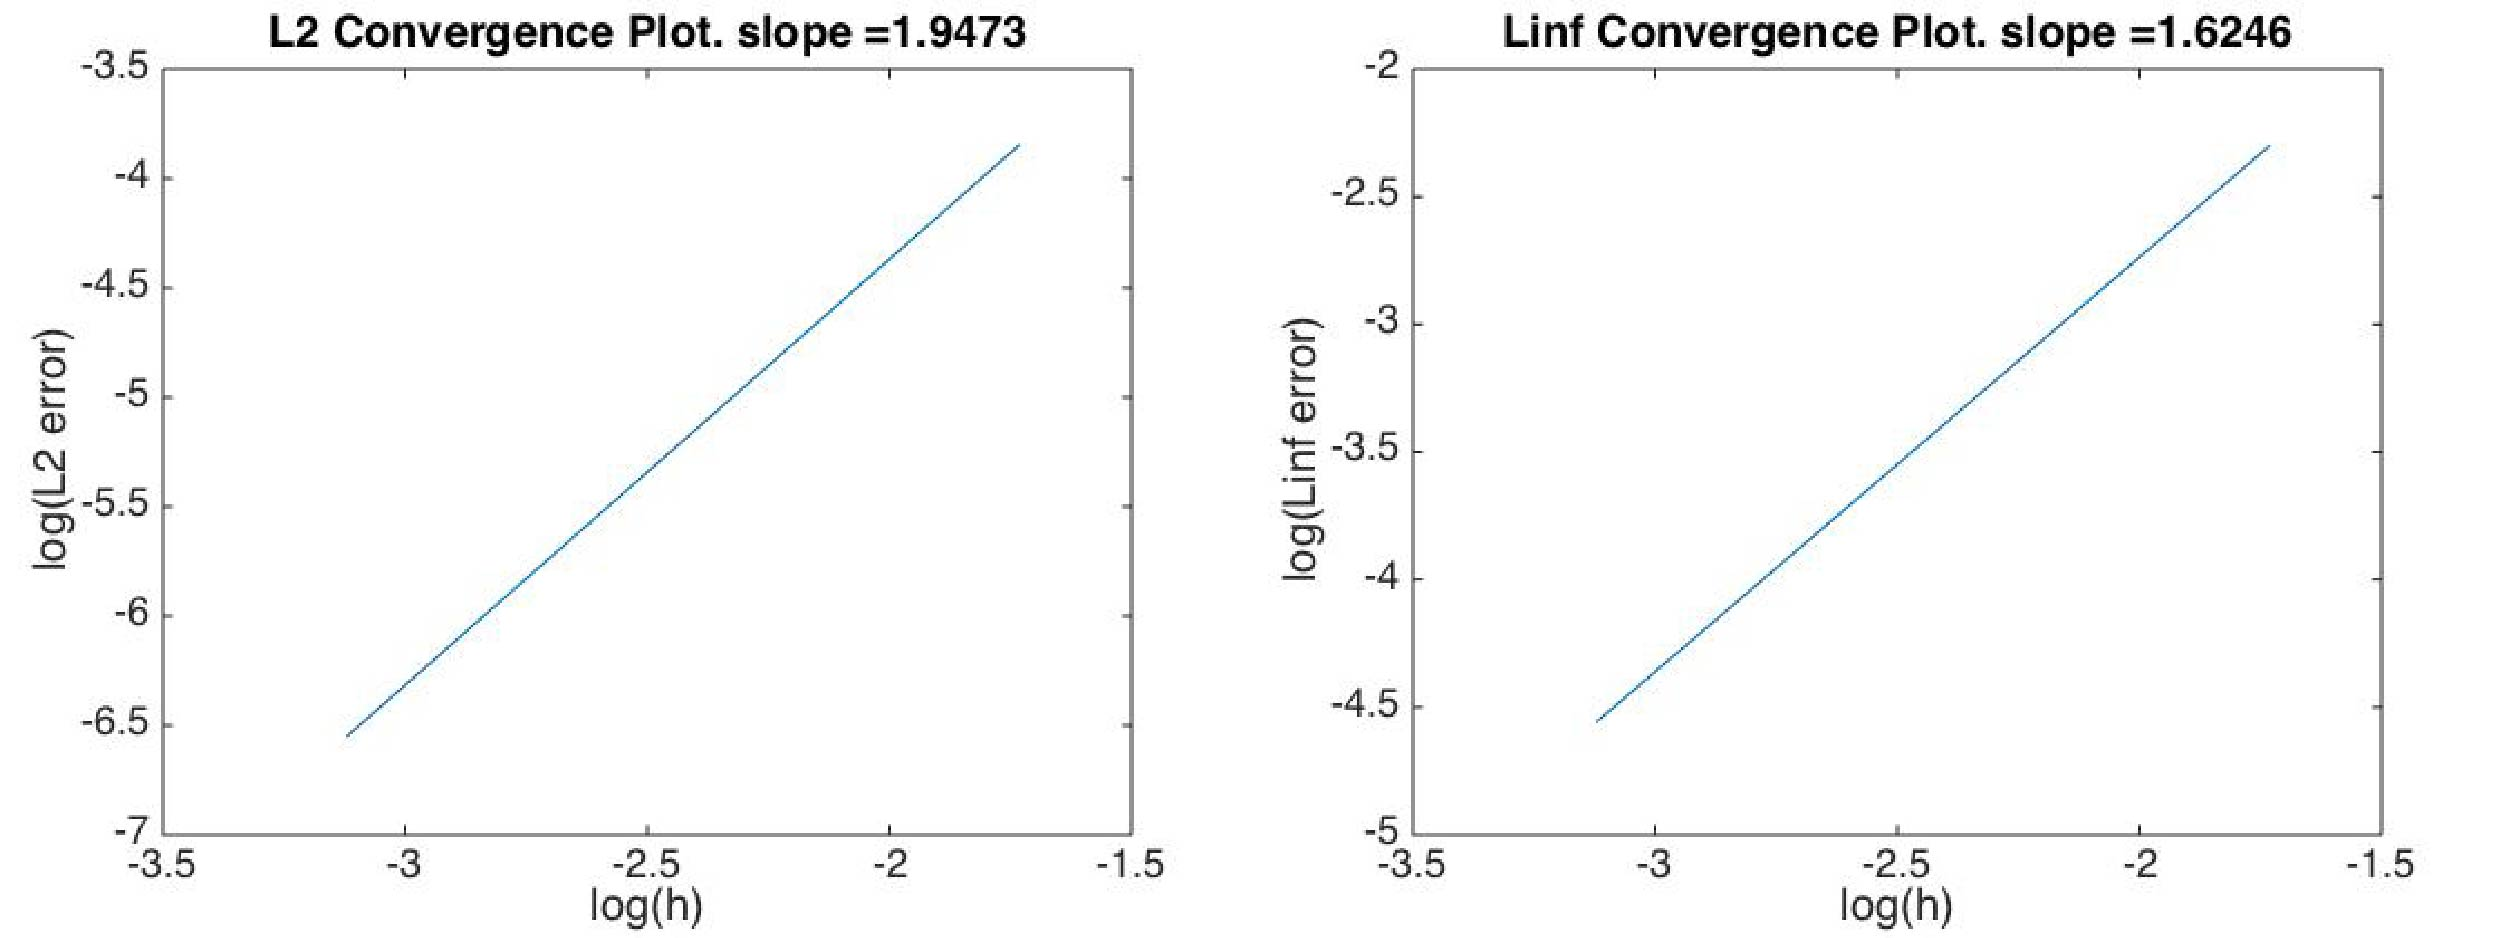
\includegraphics[width=0.9\textwidth]{2ERROR.jpg}
\end{center}

\item
The errors for this mesh are the same as the errors for the finest mesh used in part (a) (L2 = 0.0014, Linf = 0.0102), but the run time is only 2.551205 seconds. In addition, the finest mesh had 2048 elements, while this unstructured mesh has only 1286 elements. This goes to show that an unstructured mesh, if carefully designed, can yield similar numerical results to those produced on a structured mesh, but with much less computation.
\begin{center}
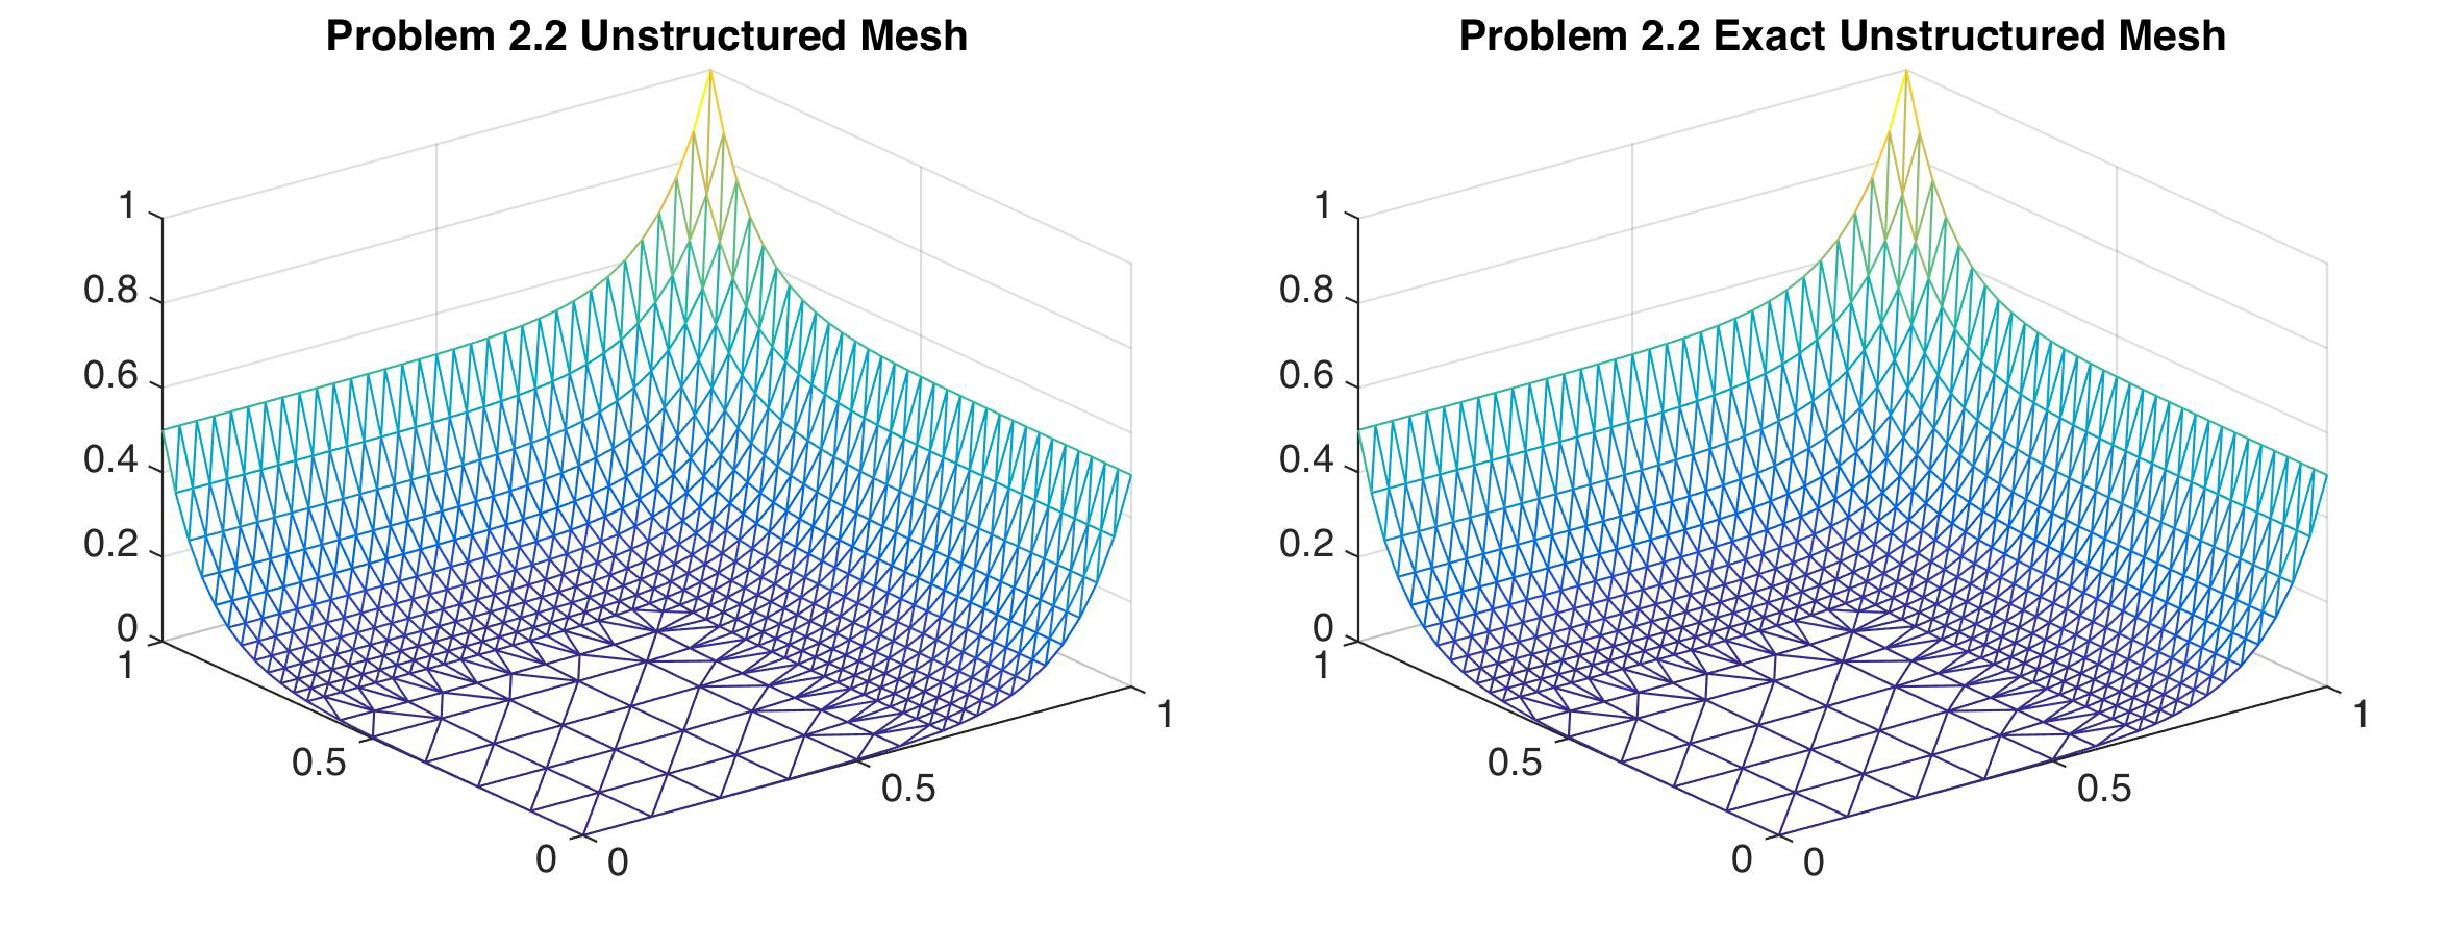
\includegraphics[width=0.9\textwidth]{22UE_.jpg}
\end{center}


\end{enumerate}

\newpage
\section*{Appendix}
\subsection*{2D FEM solver}
I had many conditional statements in the code I used to solve the problems, but I have deleted all of those and here I present a minimal working example of my code [ it is more readable this way].
\begin{lstlisting}
close all; clear all;
set(0,'DefaultAxesFontSize', 18)

% Set up a few arrays for our error plots ---------------------------------
L2arr = [];
LINFarr = []; 
Harr = [];

% Get the files we need from the appropriate directory --------------------
f = strcat('2D_Problems/Problem_2.2/um/*');
disp(f)
copyfile(f, '.')
probid = 'Problem 2.2     ';    

read_2D_mesh();
read_2D_input();
K = zeros(nnodes);
F = zeros(nnodes,1);

for n=1:nelems
    nodelist = CONN(n,:);
    x = XNODES(nodelist);
    y = YNODES(nodelist);
    k = KofXY(n);
    b = BofXY(n);
    f = FofXY(n);
    [ke, fe] = element2d(x, y, k, b, f);
    [K,F] = assemble2d(nodelist, ke, fe, K, F);
end

[K, F] = BCTYPE1(nbc1, NODEBC1, VBC1, K, F, nnodes);
[K, F] = BCType2(K, F);

% Compute and plot numerical solution ---------------------------------
u = K\F;
figure()
plt = trimesh(CONN, XNODES, YNODES, u);
ttl = strcat('Problem 2.2 Unstructured Mesh');
title(ttl);
imname = strcat('22u');
name = strcat(imname, '.jpg');
saveas(plt, name)

% Compute and plot exact solution -------------------------------------
U = exact_2D(XNODES,YNODES,probid);
figure()
trimesh(CONN, XNODES, YNODES, U)
plt2 = trimesh(CONN, XNODES, YNODES, u);
ttl = strcat('Problem 2.2 Exact Unstructured Mesh');
title(ttl);
imname = strcat('22ue');
name = strcat(imname, '.jpg');
saveas(plt2, name);

% Compute error norms -------------------------------------------------
L2 = 0;
Linf = 0;

w = [1/6, 1/6, 1/6];
p1 = @(ksi, eta) 1 - ksi - eta;
p2 = @(ksi, eta) ksi;
p3 = @(ksi, eta) eta;
psi = [p1(0.5, 0), p1(0.5, 0.5), p1(0, 0.5);...
       p2(0.5, 0), p2(0.5, 0.5), p2(0, 0.5);...
       p3(0.5, 0), p3(0.5, 0.5), p3(0, 0.5)];

for j = 1:nelems
    nodelist = CONN(j,:);
    xi = XNODES(nodelist);
    yi = YNODES(nodelist);
    h = max(max(sqrt((xi(2) - xi(1))^2 +(yi(2) - yi(1))^2 )...
              ,sqrt((xi(3) - xi(2))^2 +(yi(3) - yi(2))^2 ))...
              ,sqrt((xi(1) - xi(3))^2 +(yi(1) - yi(3))^2 ));
    ui = u(nodelist);
    A_e = 0.5*(xi(1)*yi(2) - yi(1)*xi(2) + xi(2)*yi(3) - yi(2)*xi(3) + ...
        xi(3)*yi(1) - yi(3)*xi(1));
    
    for k = [1:3]
        u_h = dot(ui, psi(:,k));
        x = dot(xi, psi(:,k));
        y = dot(yi, psi(:,k));
        U = exact_2D(x, y, probid);
        L2 = L2 + w(k) * 2*A_e*(U - u_h)^2;
        Linf = max(Linf, abs(U - u_h));
    end
end
L2 = sqrt(L2);

% Report error norms, and make error plots --------------------------------
fprintf('L2 = %d; Linf = %d;\n', L2, Linf)
LINFarr = [LINFarr, Linf];
L2arr = [L2arr, L2];
Harr = [Harr, h];

LINFarr = fliplr(log(LINFarr));
L2arr = fliplr(log(L2arr));
Harr = fliplr(log(Harr));

pl2 = polyfit(Harr, L2arr,1);
pli = polyfit(Harr, LINFarr,1);
figure();
plot(Harr, polyval(pl2, Harr));
ttl = strcat('L2 Convergence Plot. slope = ', num2str(pl2(1)));
title(ttl);
xlabel('log(h)');
ylabel('log(L2 error)')
figure();
plot(Harr, polyval(pli, Harr));
ttl = strcat('Linf Convergence Plot. slope = ', num2str(pli(1)));
title(ttl);
xlabel('log(h)');
ylabel('log(Linf error)')
\end{lstlisting}

\subsection*{element\_2d}
\begin{lstlisting}
function [ke, fe] = element2d(x, y, k, b, f)
    A_e = 0.5*(x(1)*y(2) - y(1)*x(2) + x(2)*y(3) - y(2)*x(3) + ...
        x(3)*y(1) - y(3)*x(1));% Compute area
    
    X = constructMat(x);
    Y = constructMat(y);
    
    w = [1/6, 1/6, 1/6];
    p1 = @(ksi, eta) 1 - ksi - eta;
    p2 = @(ksi, eta) ksi;
    p3 = @(ksi, eta) eta;
    psi = [p1(0.5, 0), p1(0.5, 0.5), p1(0, 0.5);...
           p2(0.5, 0), p2(0.5, 0.5), p2(0, 0.5);...
           p3(0.5, 0), p3(0.5, 0.5), p3(0, 0.5)];
       
    for i = [1:3]
        for j = [1:3]
            g_gauss = psi(i,:).*psi(j,:);
            ke(i,j) = k*(X(i,j) + Y(i,j))/(4*A_e) + ...
                2*b*A_e*dot(g_gauss, w);
        end
        fe(i) = f*A_e/3;
    end
end

function M = constructMat(m)
    M = zeros(3);
    M(1,1) = (m(2) - m(3))^2;
    M(1,2) = (m(2) - m(3))*(m(3) - m(1));
    M(2,1) = M(1,2);
    M(1,3) = (m(2) - m(3))*(m(1) - m(2));
    M(3,1) = M(1,3);
    M(2,2) = (m(3) - m(1))^2;
    M(2,3) = (m(3) - m(1))*(m(1) - m(2));
    M(3,2) = M(2,3);
    M(3,3) = (m(1) - m(2))^2;
end
\end{lstlisting}

\subsection*{assemble\_2d}
\begin{lstlisting}
function [K,F] = assemble2d(nodelist, ke, fe, K, F)
for r = [1:3]
    i = nodelist(r);
    F(i) = F(i) + fe(r);
    for s = [1:3]
        j = nodelist(s);
        K(i,j) = K(i,j) + ke(r,s);
    end
end
end
\end{lstlisting}
\end{document}
